\chapter{向量代数}

\section{向量}
数学是从认识和研究图形和数开始的。大体上可以说，图形的优点是直观形象，能更直接地用来描述我们周围的世界，也更容易理解。但图形不便于用于计算，利用几何推理的方法来研究图形，灵活性、偶然性太大，不容易掌握。数的优点是有比较死板的方法进行运算，便于掌握，但比图形更抽象，将客观世界用数来描述的难度更大一些。笛卡尔引进了坐标之后，打破了数与形的界限，将几何图形最基本的元素——点用坐标来表示，将曲线、曲面用方程来表示，通过对坐标和方程的代数运算来研究几何图形的性质，这就是解析几何。

向量也是一种图形，具有直观形象的优点，便于用来描述客观世界。向量又可以直接进行运算。因此向量兼有图形和数的优点。我们可以将几何图形用向量来描述，通过向量的运算来解决几何问题；也可以进一步将向量的运算转化为坐标的运算来解决问题，这是建立解析几何的理论与算法体系的一种简明有效的途径。

向量是一种“价廉物美”的数学工具，学起来很容易，需要花费的时间和精力不多；用处又很大，可以解决很多的几何和代数的问题。

\subsection{向量的定义}
向量，一称矢量，是一类有大小和方向的量。每个向量\(\vec{a}\)可以用一条有向线段\(A B\)来表示，记作\(\vec{a} = \vec{A B}\)。从\(A\)到\(B\)的方向表示向量\(\vec{a}\)的方向；\(A B\)的长度\(\left| A B \right|\)表示向量\(\vec{a}\)的大小，称为\(\vec{a}\)的模，记作\(\left| \vec{a} \right|\)。当\(\left| \vec{a} \right| = \left| A B \right| = 0\)时\(A\)与\(B\)重合，\(\vec{a} = \vec{A A}\)，称为零向量，记为\(\vec{0}\)。零向量的方向不确定，可以为任意方向。

同一个向量\(\vec{a}\)可以由不同的有向线段\(A B\)、\(C D\)表示，只要\(A B\)、\(C D\)的方向相同，长度也相等，即使出发点\(A\)、\(C\)不同也有\(\vec{A B} = \vec{C D}\)。但从同一点出发表示同一个向量的有向线段是唯一确定的：\(\vec{O A} = \vec{O B} \Longleftrightarrow A\)与\(B\)重合。

当非零向量\(\vec{a}\)与\(\vec{b}\)的方向相同或相反时，表示它们的有向线段既可以共线，也可以平行，此时我们称\(\vec{a} , \vec{b}\)平行（也可以称\(\vec{a} , \vec{b}\)共线）。我们规定：零向量与任意向量平行。

\subsection{向量的加法}
设\(\vec{a} , \vec{b}\)是任意两个向量。从任意一点\(O\)出发，作\(\vec{O A} = \vec{a}\)，再从\(O A\)的终点\(A\)出发作\(\vec{A B} = \vec{b}\)，则定义\(\vec{a}\)与\(\vec{b}\)相加所得的和\(\vec{a} + \vec{b} = \vec{O A} + \vec{A B} = \vec{O B}\)。向量加法的这个法则称为三角形法则。如果将\(\vec{O A} , \vec{A B}\)理解为位移，则\(\vec{O A} + \vec{A B}\)就表示两个位移的合成：\(O \to A \to B\)总的效果是由\(O\)到\(B\)，也就是\(\vec{O B}\)。

对任意3个向量\(\vec{a} , \vec{b} , \vec{c}\)作\(\vec{a} = \vec{O A} , \vec{b} = \vec{A B} , \vec{c} = \vec{B C}\)，则易见\(\left( \vec{a} + \vec{b} \right) + \vec{c} = \vec{O C} = \vec{a} + \left( \vec{b} + \vec{c} \right)\)，这也说明了向量加法的结合律成立。

设\(\vec{a} = \vec{O A}\)与\(\vec{b} = \vec{A B}\)，再作\(\vec{O C} = \vec{b}\)，连接\(C B\)。则当\(O A , A B\)不共线时，\(O A B C\)是平行四边形，从而\(\vec{C B} = \vec{O A} = \vec{a}\)，如右图所示。当\(O A , A B\)共线时，也易见\(\vec{C B} = \vec{O A}\)。因此在所有情况下都有\(\vec{b} + \vec{a} = \vec{O C} + \vec{C B} = \vec{O B} = \vec{a} + \vec{b}\)。也即向量加法交换律成立。

\begin{wrapfigure}[6]{r}{0.38\linewidth}
    \centering
    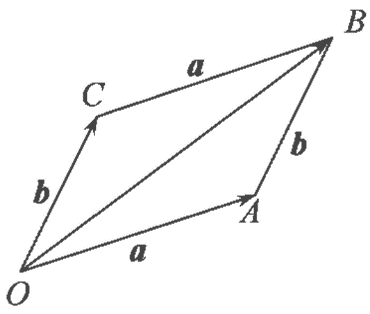
\includegraphics[width=0.84\linewidth]{image10.png}
\end{wrapfigure}

右图中的等式\(\vec{a} + \vec{b} = \vec{O A} + \vec{O C} = \vec{O B}\)给出了求向量\(\vec{a} , \vec{b}\)的和的另一个法则，称为平行四边形法则：从同一点\(O\)出发，分别作\(\vec{O A} = \vec{a} , \vec{O C} = \vec{b}\)，作平行四边形\(O A B C\)，则对角线\(\vec{O B} = \vec{a} + \vec{b}\)。

易见\(\vec{a} + \vec{0} = \vec{0} + \vec{a} = \vec{a}\)对任意向量\(\vec{a}\)成立。

对每个向量\(\vec{a} = \vec{A B}\)，存在唯一一个与\(\vec{a}\)大小相等、方向相反的向量\(\vec{B A}\)，记作\(- \vec{a}\)，也就是\(\vec{B A} = - \vec{A B}\)，称为\(\vec{a}\)的负向量。我们有\(\vec{a} + \left( - \vec{a} \right) = \vec{A B} + \vec{B A} = \vec{A A} = \vec{0} , \left( - \vec{a} \right) + \vec{a} = \vec{B A} + \vec{A B} = \vec{B B} = \vec{0}\)。反过来，\(\vec{a}\)也是\(- \vec{a}\)的负向量，即\(- \left( - \vec{a} \right) = \vec{a}\)。

向量的减法：已知向量\(\vec{a} , \vec{b}\)，定义它们的差\(\vec{a} - \vec{b} = \vec{a} + \left( - \vec{b} \right)\)，它满足条件\(\left( \vec{a} - \vec{b} \right) + \vec{b} = \vec{a}\)。从同一点\(O\)出发，分别作\(\vec{O A} = \vec{a} , \vec{O B} = \vec{b}\)，则\(\vec{a} - \vec{b} = \vec{B A}\)。

\subsection{向量与实数相乘}
任一向量\(\vec{a}\)与任一实数\(k\)可以相乘，得到一个向量，记作\(k \vec{a}\)，定义如下：

\(k \vec{a}\)的长度\(\left| k \vec{a} \right| = \left| k \right| \left| \vec{a} \right|\)。当\(k > 0\)时，\(k \vec{a}\)与\(\vec{a}\)的方向相同；当\(k < 0\)时，\(k \vec{a}\)与\(\vec{a}\)的方向相反；当\(k = 0\)时，\(k \vec{a} = \vec{0}\)是零向量，方向不确定。

由向量与实数相乘的法则知道：向量\(\vec{a} , \vec{b}\)平行\(\Leftrightarrow\)其中一个向量可以写成另一个向量与某个实数的乘积。
\newpage
如下运算律对任意向量\(\vec{a} , \vec{b}\)和实数\(k , s\)成立：

（1）\(1 \vec{a} = \vec{a} , - 1 \vec{a} = - \vec{a} , k \left( s \vec{a} \right) = \left( k s \right) \vec{a}\)；

（2）（对实数加法的分配律）\(\left( k + s \right) \vec{a} = k \vec{a} + s \vec{a}\)；

（3）（对向量加法的分配律）\(k \left( \vec{a} + \vec{b} \right) = k \vec{a} + k \vec{b}\)。

长度为\(1\)的向量称为单位向量。当\(\vec{a} \ne \vec{0}\)时，\(\frac{1}{\left| \vec{a} \right|} \vec{a}\)就是与\(\vec{a}\)方向相同的单位向量。

\begin{example}
（1）已知\(\triangle A B C\)及其两边长\(\left| A B \right| , \left| A C \right|\)。怎样用向量的语言描述：点\(P\)在\(\angle B A C\)的角平分线上。

（2）\(O\)是平面上一定点，\(A , B , C\)是平面上不共线的三个点，动点\(P\)满足\(\vec{O P} = \vec{O A} + \lambda \left( \frac{\vec{A B}}{\left| \vec{A B} \right|} + \frac{\vec{A C}}{\left| \vec{A C} \right|} \right) , \lambda \in \lbrack 0 , + \infty \rightparen\)，则\(P\)点的轨迹一定过\(\triangle A B C\)的

（A）外心 \quad （B）内心 \quad （C）重心 \quad （D）垂心
\end{example}

\subsection{向量的数量积}
任意两个向量\(\vec{a} , \vec{b}\)可以作数量积（也称内积），得到一个实数：

\(\vec{a} \cdot \vec{b} = \left| \vec{a} \right| \left| \vec{b} \right| \cos \left\langle \vec{a} , \vec{b} \right\rangle\)，其中\(\left\langle \vec{a} , \vec{b} \right\rangle\)表示\(\vec{a} , \vec{b}\)的夹角。

物理例子：设物体在恒力\(\vec{F}\)作用下沿直线前进，产生位移\(\vec{s}\)，则\(\vec{F}\)所作功\(W = \vec{F} \cdot \vec{s}\)。

有两个特殊情况值得特别注意：

（1）记\(\vec{a}^{2} = \vec{a} \cdot \vec{a}\)，由于向量\(\vec{a}\)与自身夹角为0，由\(\cos 0 = 1\)知\(\vec{a}^{2} = \left| \vec{a} \right|^{2}\)；

（2）当\(\vec{a} \perp \vec{b}\)时，\(\cos \left\langle \vec{a} , \vec{b} \right\rangle = \cos \frac{\pi}{2} = 0\)，因此\(\vec{a} \cdot \vec{b} = 0\)；我们规定零向量与所有向量垂直，这样就有\(\vec{a} \cdot \vec{b} = 0 \Longleftrightarrow \vec{a} \perp \vec{b}\)。

利用数量积可以表示任意向量\(\vec{a}\)的长度\(\left| \vec{a} \right|\)和任意两个非零向量\(\vec{a} , \vec{b}\)所成的角\(\theta\)：
\begin{equation}
    \left| \vec{a} \right| = \sqrt{\vec{a}^{2}} ; \cos \theta = \frac{\vec{a} \cdot \vec{b}}{\left| \vec{a} \right| \left| \vec{b} \right|} = \frac{\vec{a} \cdot \vec{b}}{\sqrt{\vec{a}^{2}} \sqrt{\vec{b}^{2}}}
\end{equation}

向量的数量积满足一些与数的乘法类似的运算律：

（1）\(\vec{a} \cdot \vec{b} = \vec{b} \cdot \vec{a}\)；

（2）\(\left( \vec{a} + \vec{b} \right) \cdot \vec{c} = \vec{a} \cdot \vec{c} + \vec{b} \cdot \vec{c}\)；

（3）\(\left( k \vec{a} \right) \cdot \vec{b} = k \left( \vec{a} \cdot \vec{b} \right)\)。
\newpage
\begin{example}
对任意向量\(\vec{a} , \vec{b}\)证明乘法公式\({\left( \vec{a} - \vec{b} \right)}^{2} = \vec{a}^{2} + \vec{b}^{2} - 2 \vec{a} \cdot \vec{b}\)，并对\(\vec{a} , \vec{b}\)不平行的情形解释这个公式的几何意义。
\end{example}

{\kaiti{}思考\quad 为什么这里向量的运算和数的运算可以混为一谈。}

\begin{example}
设\(A B C D\)是三维空间中的不重合的任意四个点。求证：\(A C \perp B D \Longleftrightarrow \left| A B \right|^{2} + \left| C D \right|^{2} = \left| B C \right|^{2} + \left| D A \right|^{2}\)。

\end{example}

\begin{example}
\(A B C D\)是四面体，\(\angle B A C = \angle A C D\)，\(\angle A B D = \angle B D C\)。求证：\(\left| A B \right| = \left| C D \right|\)。
\end{example}

\subsection{向量的坐标表示法}
一般地，在平面上任意选定两个相互垂直的单位向量\(\vec{\imath} , \vec{\jmath}\)，则平面内每个向量\(\vec{a} = \vec{O P}\)都可以分解为与\(\vec{\imath}\)平行的向量\(\vec{O D}\)和与\(\vec{\jmath}\)平行的向量\(\vec{D P}\)之和。\(\vec{O D} , \vec{D P}\)可以分别写成\(\vec{\imath} , \vec{\jmath}\)的实数倍\(x \vec{\imath} , y \vec{\jmath}\)。于是\(\vec{a} = \vec{O P}\)被分解成\(\vec{\imath} , \vec{\jmath}\)的实数倍之和的形式\(\vec{O P} = x \vec{\imath} + y \vec{\jmath}\)，其中的两个系数\(x , y\)由\(\vec{O P}\)唯一决定，可以认为是用\(\vec{\imath} , \vec{\jmath}\)这两个单位向量一起去“度量”\(\vec{O P}\)得到的“量数”。我们称\(\vec{\imath} , \vec{\jmath}\)组成平面上的一组基，\(\left( x , y \right)\)为\(\vec{a} = \vec{O P}\)在这组基下的坐标。坐标\(\left( x , y \right)\)唯一地代表了向量\(\vec{a}\)，我们可以直接写\(\vec{a} = \left( x , y \right)\)。将向量用坐标表示之后，向量的运算就可以转化为坐标的运算。对向量\(\vec{a} = \left( x_{1} , y_{1} \right) , \vec{b} = \left( x_{2} , y_{2} \right)\)及实数\(k\)，我们有
\begin{equation}
    \vec{a} \pm \vec{b} = \left( x_{1} \vec{\imath} + y_{1} \vec{\jmath} \right) \pm \left( x_{2} \vec{\imath} + y_{2} \vec{\jmath} \right) = \left( x_{1} \pm x_{2} \right) \vec{\imath} + \left( y_{1} \pm y_{2} \right) \vec{\jmath}
\end{equation}
\begin{equation}
    k \vec{a} = k \left( x \vec{\imath} + y \vec{\jmath} \right) = \left( k x \right) \vec{\imath} + \left( k y \right) \vec{\jmath}
\end{equation}
\begin{equation}
    \vec{a} \cdot \vec{b} = \left( x_{1} \vec{\imath} + y_{1} \vec{\jmath} \right) \cdot \left( x_{2} \vec{\imath} + y_{2} \vec{\jmath} \right) = x_{1} x_{2} + y_{1} y_{2}
\end{equation}
可以用坐标的形式简写这三个式子：
\begin{equation}
    \left( x_{1} , y_{1} \right) + \left( x_{2} , y_{2} \right) = \left( x_{1} + x_{2} , y_{1} + y_{2} \right) , k \left( x , y \right) = \left( k x , k y \right) , \left( x_{1} , y_{1} \right) \cdot \left( x_{2} , y_{2} \right) = x_{1} x_{2} + y_{1} y_{2}
\end{equation}

由向量的数量积公式立即得到：

若\(\vec{a} = \left( x , y \right)\)，则\(\left| \vec{a} \right| = \sqrt{x^{2} + y^{2}}\)；

若\(\vec{a} = \left( x_{1} , y_{1} \right) , \vec{b} = \left( x_{2} , y_{2} \right)\)，则\(\cos \left\langle \vec{a} , \vec{b} \right\rangle = \frac{x_{1} x_{2} + y_{1} y_{2}}{\sqrt{x_{1}^{2} + y_{1}^{2}} \sqrt{x_{2}^{2} + y_{2}^{2}}}\)；

向量\(\vec{a} = \left( x_{1} , y_{1} \right) , \vec{b} = \left( x_{2} , y_{2} \right)\)垂直的充分必要条件是\(x_{1} x_{2} + y_{1} y_{2} = 0\)。
\newpage
\begin{exercise}
    \mbox{}

    （1）设\(A , B , C\)是实数，且\(A , B\)不全为\(0\)，求方程\(A x + B y + C = 0\)的图像。

    （2）已知直线\(l_{1} : A_{1} x + B_{1} y + C_{1} = 0\)与\(l_{2} : A_{2} x + B_{2} y + C_{2} = 0\)。求\(l_{1} , l_{2}\)的夹角\(\theta\)以及\(l_{1} \perp l_{2}\)的充分必要条件。

    （3）已知直线\(l_{1} , l_{2}\)的斜率分别是\(k_{1} , k_{2}\)，求\(l_{1} , l_{2}\)的夹角\(\theta\)以及\(l_{1} \perp l_{2}\)的充分必要条件。

    （4）设\(\alpha\)是任意角，\(n\)是任意正整数且\(\cos \alpha + \cos 2 \alpha + \cdots + \cos n \alpha \ne 0\)。化简
    \begin{equation*}
        \frac{\sin \alpha + \sin 2 \alpha + \cdots + \sin n \alpha}{\cos \alpha + \cos 2 \alpha + \cdots + \cos n \alpha} .
    \end{equation*}
\end{exercise}

可以很自然地将二维平面的向量坐标表示扩展到三维空间上甚至更高维度上。以三维空间为例。在空间中任意取定3个两两垂直的单位向量\(\vec{\imath} , \vec{\jmath} , \vec{k}\)，则空间中每个向量\(\vec{a}\)可以唯一地写成\(\vec{a} = x \vec{\imath} + y \vec{\jmath} + z \vec{k}\)的形式，其中\(x , y , z\)是实数，\(\vec{\imath} , \vec{\jmath} , \vec{k}\)称为空间中的一组基，\(\left( x , y , z \right)\)称为\(\vec{a}\)在这组基下的坐标，可以看成是用\(\vec{\imath} , \vec{\jmath} , \vec{k}\)这一组单位向量去“度量”\(\vec{a}\)得到的“量数”。\(\vec{a}\)可以用它的坐标\(\left( x , y , z \right)\)完全代表，直接写为\(\vec{a} = \left( x , y , z \right)\)。与平面向量类似地有空间向量的坐标运算公式：
\begin{equation*}
    \left( x_{1} , y_{1} , z_{1} \right) + \left( x_{2} , y_{2} , z_{2} \right) = \left( x_{1} + x_{2} , y_{1} + y_{2} , z_{1} + z_{2} \right) , \quad k \left( x , y , z \right) = \left( k x , k y , k z \right)
\end{equation*}
\begin{equation*}
    \left( x_{1} , y_{1} , z_{1} \right) \cdot \left( x_{2} , y_{2} , z_{2} \right) = x_{1} x_{2} + y_{1} y_{2} + z_{1} z_{2} , \quad \vec{a} = \left( x , y , z \right) \to \left| \vec{a} \right| = \sqrt{x^{2} + y^{2} + z^{2}}
\end{equation*}

向量\(\vec{a} = \left( x_{1} , y_{1} , z_{1} \right) , \vec{b} = \left( x_{2} , y_{2} , z_{2} \right)\)垂直的充分必要条件是\(x_{1} x_{2} + y_{1} y_{2} + z_{1} z_{2} = 0\)。

\begin{exercise}
    \mbox{}

    \noindent\begin{minipage}[t]{0.58\linewidth}
    \setlength{\parindent}{2em}\setlength{\parskip}{6pt}
    已知正方体\(A B C D - A^{'} B^{'} C^{'} D^{'}\)如图，求：

    （1）直线\(A B\)与平面\(B D A^{'}\)所成的角；

    （2）平面\(A^{'} B^{'} C D\)与\(B D D^{'} B^{'}\)的夹角。
    \end{minipage}\hfill
    \begin{minipage}[t]{0.34\linewidth}
    \centering
    \adjustbox{valign=t}{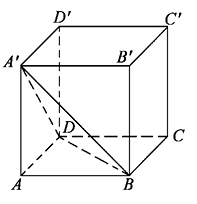
\includegraphics[width=0.92\linewidth]{image11.png}}
    \end{minipage}
\end{exercise}

\newpage

\section{三维空间中的几何关系}
三维空间中的几何关系主要包含点、线、面之间的位置关系，主要涉及距离、夹角等度量关系。为叙述方便，以下几何关系将在笛卡尔直角坐标系下使用向量语言进行叙述。对于其他坐标系下的描述这里暂不涉及，可由坐标变换关系自行推导。

\subsection{点与点的关系}
点与点的关系较为简单，一般考虑两点间的距离公式：若空间中两点\(A , B\)坐标分别为\(A \left( x_{1} , y_{1} , z_{1} \right) , B \left( x_{2} , y_{2} , z_{2} \right)\)，则\(\left| A B \right| = \left| \vec{A B} \right| = \left| \left( x_{2} - x_{1} , y_{2} - y_{1} , z_{2} - z_{1} \right) \right| = \sqrt{{\left( x_{2} - x_{1} \right)}^{2} + {\left( y_{2} - y_{1} \right)}^{2} + {\left( z_{2} - z_{1} \right)}^{2}}\)。

\subsection{点与线的关系}
如果点\(P\)的坐标为\(\left( x_{0} , y_{0} , z_{0} \right)\)，直线\(L\)的方向向量为\(\vec{l} = \left( a , b , c \right)\)，且直线上有一点\(Q\)的坐标为\(\left( x_{1} , y_{1} , z_{1} \right)\)，则点\(P\)到直线\(L\)的距离\(d\)为：
\begin{equation}
    d = \frac{\left| \vec{P Q} \times \vec{l} \right|}{\left| \vec{l} \right|}
    = \sqrt{\left| \vec{P Q} \right|^{2} - \frac{\left( \vec{P Q} \cdot \vec{l} \right)^{2}}{\left| \vec{l} \right|^{2}}}
\end{equation}

其中\(\vec{P Q} = \left( x_{1} - x_{0} , y_{1} - y_{0} , z_{1} - z_{0} \right)\)。定义两个三维向量\(\vec{a} , \vec{b}\)的外积\(\vec{a} \times \vec{b}\)（一称向量积）：两个三维向量的外积为一个向量，其模长为\(\left| \vec{a} \right| \left| \vec{b} \right| \sin \left\langle \vec{a} , \vec{b} \right\rangle\)，方向垂直于\(\vec{a} , \vec{b}\)，按从\(\vec{a}\)到\(\vec{b}\)的右手定则确定方向（当\(\vec{a} \parallel \vec{b}\)时，规定\(\vec{a} \times \vec{b} = \vec{0}\)）。

\subsection{点与面的关系}
如果点\(P\)的坐标为\(\left( x_{0} , y_{0} , z_{0} \right)\)，平面\(\pi\)的方程为\(A x + B y + C z + D = 0\)（\(A , B , C\)不全为0），则\(P\)到平面\(\pi\)的距离\(d\)为：
\begin{equation}
    d = \frac{\left| A x_{0} + B y_{0} + C z_{0} + D \right|}{\sqrt{A^{2} + B^{2} + C^{2}}}
\end{equation}

\subsection{线与线的关系}
如果两直线的方向向量分别为\(\vec{d}_{1} = \left( a_{1} , b_{1} , c_{1} \right)\)和\(\vec{d}_{2} = \left( a_{2} , b_{2} , c_{2} \right)\)，则两直线夹角\(\theta \in [0 , \frac{\pi}{2}]\)的余弦值为：
\begin{equation}
    \cos \theta = \frac{\left| \vec{d}_{1} \cdot \vec{d}_{2} \right|}{\left| \vec{d}_{1} \right| \left| \vec{d}_{2} \right|}
\end{equation}

\subsection{线与面的关系}
如果直线的方向向量为\(\vec{d} = \left( a , b , c \right)\)，平面的法向量为\(\vec{n} = \left( A , B , C \right)\)，则直线与平面的夹角\(\theta \in [0 , \frac{\pi}{2}]\)的正弦值为：
\begin{equation}
    \sin \theta = \frac{\left| \vec{d} \cdot \vec{n} \right|}{\left| \vec{d} \right| \left| \vec{n} \right|}
\end{equation}

\subsection{面与面的关系}
如果两平面的法向量分别为\(\vec{n}_{1} = \left( a_{1} , b_{1} , c_{1} \right)\)和\(\vec{n}_{2} = \left( a_{2} , b_{2} , c_{2} \right)\)，则两平面夹角\(\theta \in [0 , \frac{\pi}{2}]\)的余弦值为：
\begin{equation}
    \cos \theta = \frac{\left| \vec{n}_{1} \cdot \vec{n}_{2} \right|}{\left| \vec{n}_{1} \right| \left| \vec{n}_{2} \right|}
\end{equation}

于是可以容易地将三维空间中的线、面之间的平行、垂直等几何关系使用向量语言进行描述：

面与面平行/垂直：其法向量平行/垂直。

线与线平行/垂直：其方向向量平行/垂直。

线与面平行/垂直：线的方向向量与面的法向量垂直/平行。

因此，常见立体几何的题目的一般做法为：

第一步：建立合适的坐标系，使得题目所涉及各点坐标尽可能简单。

第二步：将待求几何量（一般为角度）或待证明几何关系用向量语言进行描述。

第三步：求相关向量的坐标表示。

（a）直线的方向向量：直接选取直线上已知的两点坐标计算；

（b）平面的法向量：

1）设其法向量为\(\vec{n} = \left( x , y , z \right)\)，利用平面已知的三点构建在该平面内的两个不平行的向量\(\vec{\alpha} , \vec{\beta}\)（或其他点，总的原则是选取使向量的坐标表示尽可能简单的点）。

2）列式计算\(\vec{n} \cdot \vec{\alpha} = 0\)和\(\vec{n} \cdot \vec{\beta} = 0\)，令\(x\)（或\(y , z\)）为一个合适的值（总的原则是选取容易求解方程的值，或者使\(\vec{n}\)成为单位向量），求出该平面的一个法向量。

第四步：将第三步得到的向量坐标代入第二步的向量语言描述中，进行相关的运算或列方程/等式，完成证明。

\section{线性空间*}
在前面的讨论中，向量的运算可以转化为坐标的运算。例如，两个平面向量相加，就是将它们的横、纵坐标分别相加；向量与实数相乘，就是将各个坐标同乘这个实数。这样的运算也可以用于三个、四个乃至任意有限多个数所组成的数组，而不必先为它们找一个几何图形。

函数也有类似的运算。设\(f , g\)都是定义在\(\mathbb{R}\)上的实值函数，规定
\begin{equation}
    \left( f + g \right) \left( x \right) = f \left( x \right) + g \left( x \right) , \quad \left( k f \right) \left( x \right) = k f \left( x \right) .
\end{equation}
容易知道，函数的加法与数乘满足和几何向量相同的运算律。进一步地，一个二次多项式可以写成\(a + b x + c x^{2}\)，正如一个空间向量可以写成\(a \vec{\imath} + b \vec{\jmath} + c \vec{k}\)：都是选取几个固定的对象，将它们分别乘以一个数再相加。

数组、函数与几何向量是不同的对象，但只要研究中用到的是共同的运算规律，就可以用同样的方法处理。将这些规律提炼出来，就得到线性空间的概念。

\subsection{线性空间的定义}
\begin{definition}\label{def:linspace}
设\(V\)是一个集合，在\(V\)上规定了加法与数乘：对任意\(a , b \in V\)，有\(a + b \in V\)；对任意实数\(k\)和\(a \in V\)，有\(k a \in V\)。如果对任意\(a , b , c \in V\)和实数\(k , s\)，下列运算律成立：

（1）\(a + b = b + a\)；

（2）\(\left( a + b \right) + c = a + \left( b + c \right)\)；

（3）存在零向量\(\vec{0}\)，使\(a + \vec{0} = a\)；

（4）每个\(a\)都有负向量\(- a\)，使\(a + \left( - a \right) = \vec{0}\)；

（5）\(1 a = a\)；

（6）\(k \left( s a \right) = \left( k s \right) a\)；

（7）\(k \left( a + b \right) = k a + k b\)；

（8）\(\left( k + s \right) a = k a + s a\)，

则称\(V\)为一个实线性空间，也称实向量空间，\(V\)中的元素统称为向量。
\end{definition}

这里的“向量”有了更一般的含义，它可以是几何向量，也可以是数组、函数等对象。线性空间只规定加法与数乘及其运算律，长度与夹角则需要另行规定。本节和下一节的数乘都以实数为标量。

全体\(n\)元实数组组成的集合记为\(\mathbb{R}^{n}\)，按分量规定加法与数乘：
\begin{equation}
    \left( x_{1} , \ldots , x_{n} \right) + \left( y_{1} , \ldots , y_{n} \right) = \left( x_{1} + y_{1} , \ldots , x_{n} + y_{n} \right) ,
\end{equation}
\begin{equation}
    k \left( x_{1} , \ldots , x_{n} \right) = \left( k x_{1} , \ldots , k x_{n} \right) .
\end{equation}
由实数的运算律，容易验证它是一个线性空间。平面向量与空间向量的坐标运算，分别就是\(\mathbb{R}^{2}\)和\(\mathbb{R}^{3}\)中的运算。

定义在\(\mathbb{R}\)上的全体实值函数，在本节开头规定的运算下，也构成线性空间。其中零向量是恒等于零的函数，\(f\)的负向量是函数\(- f\)。类似地，全体数列也构成线性空间，其运算按每一项进行。

{\kaiti{}思考\quad 只用上述运算律证明：零向量与负向量都是唯一的，并且\(0 a = \vec{0}\)，\(\left( - 1 \right) a = - a\)。}

\subsection{子空间}
平面上过原点的一条直线，在向量的加法与数乘下，自身也构成线性空间；空间中过原点的平面也有同样的性质。这些较小的线性空间都包含在原来的线性空间中。

\begin{definition}\label{def:subspace}
设\(U\)是线性空间\(V\)的一个子集。如果\(U\)在\(V\)的加法与数乘下也构成线性空间，则称\(U\)为\(V\)的子空间。
\end{definition}

判断子空间，只需验证它含零向量，并且对加法、数乘封闭。其余运算律由\(V\)中的运算律直接得到，负向量则由\(- a = \left( - 1 \right) a\)得到。因此，判据也可以写成：\(U\)非空，且对任意\(a , b \in U\)与实数\(k , s\)，都有\(k a + s b \in U\)。

例如，在\(\mathbb{R}^{3}\)中，满足\(x + y - z = 0\)的数组组成一个子空间，几何上就是一个过原点的平面。把方程右边改成\(1\)，所得平面不含零向量，也就不再是子空间。

一般地，形如
\begin{equation}
    \left\{ \begin{matrix}
        a_{11} x_{1} + \cdots + a_{1 n} x_{n} = b_{1} , \\
        a_{21} x_{1} + \cdots + a_{2 n} x_{n} = b_{2} , \\
        \cdots \cdots \cdots \\
        a_{m 1} x_{1} + \cdots + a_{m n} x_{n} = b_{m}
    \end{matrix} \right.
\end{equation}
的方程组称为{\heiti{}线性方程组}。其中\(x_{1} , \ldots , x_{n}\)是未知量，\(a_{i j}\)为系数，\(b_{i}\)为常数项。常数项全为零时，称为{\heiti{}齐次线性方程组}。

齐次线性方程组的解集是\(\mathbb{R}^{n}\)的一个子空间。事实上，若\(u , v\)都是解，则对每个方程都有
\begin{equation}
    \sum_{j = 1}^{n} a_{i j} \left( u_{j} + v_{j} \right)
    = \sum_{j = 1}^{n} a_{i j} u_{j} + \sum_{j = 1}^{n} a_{i j} v_{j} = 0 .
\end{equation}
所以\(u + v\)仍是解，同理\(k u\)也是解，而零向量显然是解。

函数空间中的例子也很多。定义在\(\mathbb{R}\)上的全体奇函数、全体偶函数分别构成子空间；次数不超过\(2\)的实系数多项式连同零多项式也构成一个子空间，记为\(P_{2}\)。这些集合对加法与数乘的封闭性都容易验证。

{\kaiti{}思考\quad 两个子空间的交集还是子空间吗？它们的并集呢？}

\subsection{线性组合与线性无关}
设\(a_{1} , \ldots , a_{m}\)是线性空间中的一组向量。形如
\begin{equation}
    k_{1} a_{1} + k_{2} a_{2} + \cdots + k_{m} a_{m}
\end{equation}
的向量称为这组向量的一个{\heiti{}线性组合}。若\(a\)可以写成上述形式，就称\(a\)可以由\(a_{1} , \ldots , a_{m}\)线性表示。

记\(\operatorname{span}\left( a_{1} , \ldots , a_{m} \right)\)为这组向量的一切线性组合组成的集合，称为由它们{\heiti{}张成的子空间}。两个线性组合相加，或将一个线性组合乘以实数，所得结果仍是线性组合，因此子空间判据直接成立。

在\(\mathbb{R}^{3}\)中，取\(a_{1} = \left( 1 , 0 , 1 \right)\)，\(a_{2} = \left( 0 , 1 , 1 \right)\)。要将\(\left( x , y , z \right)\)表示为\(k_{1} a_{1} + k_{2} a_{2}\)，就是求解
\begin{equation}
    k_{1} = x , \quad k_{2} = y , \quad k_{1} + k_{2} = z .
\end{equation}
所以能被表示的向量恰好满足\(x + y - z = 0\)，也就是前面的平面子空间。可见，求线性表示与解线性方程组是同一个计算问题。

有了表示，进一步的问题就是表示是否唯一。如果同一个向量有两种表示，
\begin{equation}
    k_{1} a_{1} + \cdots + k_{m} a_{m} = s_{1} a_{1} + \cdots + s_{m} a_{m} ,
\end{equation}
相减可得
\begin{equation}
    \left( k_{1} - s_{1} \right) a_{1} + \cdots + \left( k_{m} - s_{m} \right) a_{m} = \vec{0} .
\end{equation}
因此，只需研究零向量的表示：如果零向量只能由系数全为零的组合表示，任意向量的表示就都是唯一的。

\begin{definition}\label{def:linindep}
设\(a_{1} , \ldots , a_{m}\)是线性空间中的一组向量。如果
\begin{equation}
    k_{1} a_{1} + \cdots + k_{m} a_{m} = \vec{0}
\end{equation}
只能在\(k_{1} = \cdots = k_{m} = 0\)时成立，则称这组向量线性无关；否则称它们线性相关。
\end{definition}

线性相关意味着存在一组不全为零的系数使上述等式成立。取其中\(k_{j} \ne 0\)的一项，移项并除以\(k_{j}\)，即可将\(a_{j}\)表示为其余向量的线性组合。反过来，若其中一个向量可由其余向量线性表示，移项就得到一个系数不全为零的零组合。因此，一组向量线性相关，当且仅当其中某个向量可由其余向量线性表示。

这也说明，线性相关的向量组可以删去其中某个向量，而不改变张成的子空间。例如，向上面的向量组中加入\(a_{3} = \left( 1 , 1 , 2 \right)\)，由于\(a_{3} = a_{1} + a_{2}\)，所能表示的向量没有增加，表示却不再唯一：
\begin{equation}
    k_{1} a_{1} + k_{2} a_{2}
    = \left( k_{1} - t \right) a_{1} + \left( k_{2} - t \right) a_{2} + t a_{3} .
\end{equation}

在几何向量中，两个向量线性相关就是共线，三个向量线性相关就是共面。在坐标中，判断线性无关就是判断相应的齐次线性方程组是否只有零解。两种语言描述的是同一个关系。

\begin{example}
（1）判断向量组\(\left( 1 , 0 , 1 \right)\)，\(\left( 0 , 1 , 1 \right)\)，\(\left( 1 , 1 , 0 \right)\)是否线性无关。

（2）在函数空间中，证明\(\sin x , \cos x\)线性无关，而\(1 , \sin^{2} x , \cos^{2} x\)线性相关。

（3）设\(a , b , c\)线性无关，证明\(a + b , b + c , c + a\)线性无关。逆命题是否成立？
\end{example}

\subsection{基与坐标}
为了用一组向量表示整个空间，需要它们张成这个空间；为了让表示唯一，又需要它们线性无关。将这两个要求放在一起，就得到基的概念。

\begin{definition}\label{def:basis}
设\(e_{1} , \ldots , e_{n}\)是线性空间\(V\)中的一组向量。如果它们线性无关，并且张成\(V\)，则称它们为\(V\)的一组基。
\end{definition}

由前面的讨论，\(e_{1} , \ldots , e_{n}\)是一组基，当且仅当\(V\)中的每个向量\(a\)都可以唯一地写成
\begin{equation}
    a = x_{1} e_{1} + x_{2} e_{2} + \cdots + x_{n} e_{n} .
\end{equation}
这里唯一确定的数组\(\left( x_{1} , \ldots , x_{n} \right)\)称为\(a\)在这组基下的坐标。

前面选取互相垂直的单位向量建立坐标，是这里的一种特殊情形。建立坐标的基本要求是表示的存在性与唯一性，因此也可以用其他的基。例如，在\(\mathbb{R}^{2}\)中取
\(e_{1} = \left( 1 , 1 \right)\)，\(e_{2} = \left( 1 , 2 \right)\)。由
\begin{equation}
    \left( x , y \right) = s e_{1} + t e_{2}
\end{equation}
得到\(s + t = x\)，\(s + 2 t = y\)，故\(s = 2 x - y\)，\(t = y - x\)。任意向量都有唯一的表示，所以它们是一组基。\(\left( 3 , 4 \right) = 2 e_{1} + e_{2}\)在这组基下的坐标是\(\left( 2 , 1 \right)\)，在通常的正交单位基下则是\(\left( 3 , 4 \right)\)。同一个向量，换一组基，坐标一般也随之改变。

在\(P_{2}\)中，\(1 , x , x^{2}\)是一组基，多项式\(a + b x + c x^{2}\)的坐标是\(\left( a , b , c \right)\)。取定一组基，就将多项式的加法、数乘转化为系数的运算。

一般地，如果\(a , b\)的坐标分别为\(\left( x_{1} , \ldots , x_{n} \right)\)与\(\left( y_{1} , \ldots , y_{n} \right)\)，则
\begin{equation}
    k a + s b = \sum_{i = 1}^{n} \left( k x_{i} + s y_{i} \right) e_{i} .
\end{equation}
因此它的坐标就是\(\left( k x_{1} + s y_{1} , \ldots , k x_{n} + s y_{n} \right)\)。这说明，取定一组基之后，向量的加法与数乘都化为\(\mathbb{R}^{n}\)中的运算。

{\kaiti{}思考\quad 在上面的基\(e_{1} , e_{2}\)下，若两个向量的坐标分别为\(\left( s_{1} , t_{1} \right)\)与\(\left( s_{2} , t_{2} \right)\)，它们的数量积还是\(s_{1} s_{2} + t_{1} t_{2}\)吗？请写出正确的式子。}

\subsection{维数}
同一个空间可以有不同的基，那么一组基所含向量的个数会不会改变？平面的基总是含两个向量，空间的基总是含三个向量。这种不随基改变的性质，在一般线性空间中也成立。

\begin{theorem}\label{thm:dim}
设\(e_{1} , \ldots , e_{n}\)与\(f_{1} , \ldots , f_{m}\)是同一个线性空间的两组基，则\(n = m\)。
\end{theorem}

{\heiti{}证明思路：}
\nopagebreak[4]

线性无关的向量组没有可以删去的向量，而张成空间的向量组已经足以表示所有向量。因此，如果一组线性无关的向量都能由另一组向量表示，前者的个数就不应超过后者。证明这个事实，可以逐个将线性无关的向量换入原来的向量组，并保持所张成的空间不变。

{\heiti{}证明：}
\nopagebreak[4]

设\(u_{1} , \ldots , u_{p}\)线性无关，且都能由\(w_{1} , \ldots , w_{q}\)表示。记\(W = \operatorname{span}\left( w_{1} , \ldots , w_{q} \right)\)。先将\(u_{1}\)表示为\(w\)组的线性组合，由于\(u_{1} \ne \vec{0}\)，至少有一个系数不为零。不妨设\(w_{1}\)的系数不为零，则可以反过来将\(w_{1}\)表示为\(u_{1} , w_{2} , \ldots , w_{q}\)的线性组合。因此，用\(u_{1}\)替换\(w_{1}\)后，张成的空间仍是\(W\)。

假设已经换入\(u_{1} , \ldots , u_{k - 1}\)，现在将\(u_{k}\)用当前向量组表示。如果剩下的\(w\)的系数全为零，就将\(u_{k}\)表示为前面几个\(u\)的线性组合，与线性无关矛盾。因此仍有某个\(w\)的系数不为零，可以将它替换为\(u_{k}\)，并保持张成的空间不变。

每次替换，\(u\)多一个而\(w\)少一个。如果\(p > q\)，经过\(q\)次替换后，\(u_{1} , \ldots , u_{q}\)已经张成\(W\)，于是\(u_{q + 1}\)可由它们表示，仍与线性无关矛盾。故\(p \le q\)。

现在将这个事实用于两组基。因为\(e\)组线性无关，且每个\(e_{i}\)都可由\(f\)组表示，所以\(n \le m\)；交换两组的角色，又得\(m \le n\)，故\(n = m\)。

能由有限个向量张成的线性空间称为{\heiti{}有限维线性空间}。从一组有限的张成向量中逐次删去可以由其余向量表示的向量，就得到一组基。这组基中向量的个数称为空间的{\heiti{}维数}，记为\(\dim V\)。上面的定理保证维数不依赖于基的选择。

例如，\(\mathbb{R}^{n}\)的标准基
\begin{equation}
    e_{1} = \left( 1 , 0 , \ldots , 0 \right) , \quad
    e_{2} = \left( 0 , 1 , \ldots , 0 \right) , \quad \ldots , \quad
    e_{n} = \left( 0 , \ldots , 0 , 1 \right)
\end{equation}
含有\(n\)个向量，所以\(\dim \mathbb{R}^{n} = n\)。\(P_{2}\)的基\(1 , x , x^{2}\)含三个向量，所以它也是三维空间。前面平面\(x + y - z = 0\)中的\(a_{1} , a_{2}\)是一组基，因此这个子空间的维数是\(2\)。维数所计数的是一组基中的向量，也就是描述空间中任意向量所需的坐标个数。

在\(n\)维空间中，线性无关的向量组至多含\(n\)个向量。若已有一组线性无关的向量而它们尚未张成整个空间，就选取一个不能由它们表示的向量加入，所得向量组仍线性无关。这样继续添加，至多达到\(n\)个向量，就得到一组基。因此，任意线性无关的向量组都可以补成一组基，特别地，\(n\)个线性无关的向量已经是一组基。

对子空间也可以这样选取向量，至多经过\(n\)次就得到它的一组基。因此，有限维空间的子空间仍然有限维，并且维数不超过原空间。

也有不能由有限个向量张成的线性空间，称为{\heiti{}无限维线性空间}。例如，全体实系数多项式组成的空间就是无限维的：任取有限个多项式，总能找到一个非负整数\(d\)，使它们的次数都不超过\(d\)，则它们的任何线性组合都不能得到\(x^{d + 1}\)。所以任意有限组多项式都不能张成整个多项式空间。

{\kaiti{}思考\quad 定义在\(\mathbb{R}\)上的全体实值函数组成的空间，是有限维的吗？}

\begin{exercise}
（1）判断下列\(\mathbb{R}^{3}\)的子集是否为子空间：\\
（a）\(\left\{ \left( x , y , z \right) \mid x + y + z = 0 \right\}\)；\\
（b）\(\left\{ \left( x , y , z \right) \mid x + y + z = 1 \right\}\)；\\
（c）\(\left\{ \left( x , y , z \right) \mid x y = 0 \right\}\)；\\
（d）\(\left\{ \left( x , y , z \right) \mid x = 2 y , z = 3 y \right\}\)。\\
对其中的子空间，求一组基及其维数。

（2）设\(a_{1} = \left( 1 , 0 , 1 \right)\)，\(a_{2} = \left( 0 , 1 , 1 \right)\)，\(a_{3} = \left( 1 , 1 , t \right)\)。讨论\(t\)取何值时，这组向量线性无关。

（3）在\(\mathbb{R}^{2}\)中，验证\(e_{1} = \left( 1 , 2 \right)\)，\(e_{2} = \left( 1 , 3 \right)\)构成一组基，并求\(\left( 4 , 7 \right)\)在这组基下的坐标。

（4）判断\(\left( 17 , - 4 , 2 \right)\)和\(\left( 17 , - 4 , 5 \right)\)能否由\(\left( 2 , 1 , - 3 \right)\)，\(\left( 1 , - 2 , 4 \right)\)线性表示；如果能，求出表示式。

（5）求齐次线性方程组
\begin{equation}
    \left\{ \begin{matrix}x + y + z = 0 , \\ x - y + z = 0\end{matrix} \right.
\end{equation}
的解集的一组基及其维数。

（6）在\(P_{2}\)中，判断\(1 , x + 1 , \left( x + 1 \right)^{2}\)是否构成一组基。若构成，求\(x^{2}\)在这组基下的坐标。

（7）证明：每个定义在\(\mathbb{R}\)上的实值函数都可以唯一地表示为一个奇函数与一个偶函数之和。

（8）在正实数集上规定\(u \oplus v = u v\)，\(k \odot u = u^{k}\)。验证它在这两种运算下是实线性空间，并求一组基及其维数。
\end{exercise}
\newpage


\section{线性变换*}
有了向量的加法与数乘，就可以用线性组合描述空间中的向量。现在考虑空间之间的映射：如果先做线性组合再进行映射，与先进行映射再做同样的线性组合，所得结果一致，这样的映射就保持了线性空间的运算结构。

\subsection{线性变换}
\begin{definition}\label{def:linmap}
设\(V , W\)是实线性空间。如果映射\(T : V \longrightarrow W\)对任意\(a , b \in V\)和实数\(k , s\)都满足
\begin{equation}
    T \left( k a + s b \right) = k T \left( a \right) + s T \left( b \right) ,
\end{equation}
则称\(T\)为线性映射，也称线性变换。当\(W = V\)时，称为\(V\)上的线性变换。
\end{definition}

上式也可以分为两个要求：可加性\(T \left( a + b \right) = T \left( a \right) + T \left( b \right)\)与齐次性\(T \left( k a \right) = k T \left( a \right)\)。自然地，线性变换将零向量映为零向量，并且保持任意有限个向量的线性组合。

例如，平面上的伸缩\(T \left( x , y \right) = \left( 2 x , 3 y \right)\)是线性变换，\(T \left( x , y \right) = \left( x + y , y \right)\)也是线性变换。前者将单位圆变成椭圆，后者将单位正方形变成平行四边形。

线性变换还与直线有直接联系。将直线上的点写成\(a + t b\)，则
\begin{equation}
    T \left( a + t b \right) = T \left( a \right) + t T \left( b \right) .
\end{equation}
所以直线的像仍是直线，或在\(T \left( b \right) = \vec{0}\)时成为一个点。线性变换的定义从运算出发，而直线、平面等几何对象的变化也就随之确定。

{\kaiti{}思考\quad 平移\(T \left( a \right) = a + b\)（\(b \ne \vec{0}\)）为什么不是线性变换？}

\subsection{线性变换的矩阵表示}
一组基能够表示整个空间，因此，要确定一个线性变换，只需知道这组基中的向量被映到哪里。

\begin{theorem}\label{thm:linmap-basis}
设\(e_{1} , \ldots , e_{n}\)是\(V\)的一组基，则线性映射\(T : V \longrightarrow W\)由\(T \left( e_{1} \right) , \ldots , T \left( e_{n} \right)\)完全决定。反过来，任意给定\(w_{1} , \ldots , w_{n} \in W\)，都恰好确定一个满足\(T \left( e_{j} \right) = w_{j}\)的线性映射。
\end{theorem}

证明是直接的。将任意向量写成\(a = x_{1} e_{1} + \cdots + x_{n} e_{n}\)，由线性性有
\begin{equation}\label{eq:linmap-basis-expansion}
    T \left( a \right) = x_{1} T \left( e_{1} \right) + \cdots + x_{n} T \left( e_{n} \right) .
\end{equation}
所以基向量的像确定后，任意向量的像都确定了。反过来，任取\(w_{1} , \ldots , w_{n} \in W\)，按\(T \left( a \right) = x_{1} w_{1} + \cdots + x_{n} w_{n}\)规定映射，坐标的唯一性保证它有确定的意义，且由坐标的运算容易验证它是线性的。

当\(W\)也是有限维空间时，取它的一组基\(f_{1} , \ldots , f_{m}\)，将每个像\(T \left( e_{j} \right)\)写成坐标形式：
\begin{equation}
    T \left( e_{j} \right) = a_{1 j} f_{1} + a_{2 j} f_{2} + \cdots + a_{m j} f_{m} .
\end{equation}
将这些坐标按列排列，得到
\begin{equation}
    A = \left[ \begin{matrix}
        a_{11} & a_{12} & \cdots & a_{1 n} \\
        a_{21} & a_{22} & \cdots & a_{2 n} \\
        \vdots & \vdots & & \vdots \\
        a_{m 1} & a_{m 2} & \cdots & a_{m n}
    \end{matrix} \right] .
\end{equation}
这样的长方形数表称为{\heiti{}矩阵}，这里有\(m\)行、\(n\)列，称为\(m \times n\)矩阵。它就是\(T\)在所选两组基下的矩阵。

将式\eqref{eq:linmap-basis-expansion}中的各个像用坐标展开，得到
\begin{equation}
    T \left( a \right)
    = \sum_{i = 1}^{m} \left( \sum_{j = 1}^{n} a_{i j} x_{j} \right) f_{i} .
\end{equation}
所以，如果\(T \left( a \right)\)的坐标为\(\left( y_{1} , \ldots , y_{m} \right)\)，就有\(y_{i} = \sum_{j = 1}^{n} a_{i j} x_{j}\)。将坐标写成列的形式，分别记为\(X , Y\)，便可以记作
\begin{equation}
    Y = A X .
\end{equation}
例如二维情况下，这个运算就是
\begin{equation}
    \left[ \begin{matrix}y_{1} \\ y_{2}\end{matrix} \right]
    = \left[ \begin{matrix}a_{11} & a_{12} \\ a_{21} & a_{22}\end{matrix} \right]
      \left[ \begin{matrix}x_{1} \\ x_{2}\end{matrix} \right]
    = \left[ \begin{matrix}a_{11} x_{1} + a_{12} x_{2} \\ a_{21} x_{1} + a_{22} x_{2}\end{matrix} \right] .
\end{equation}
矩阵与坐标列的乘法规则，就是由线性变换自然导出的。求一个线性变换的矩阵，基本方法也是求各个基向量的像，将它们的坐标按列排列。矩阵表示依赖于基的选择，同一个变换在不同基下的矩阵一般不同。

\begin{example}
设\(T\)是\(\mathbb{R}^{2}\)上的线性变换，已知\(T \left( 1 , 0 \right) = \left( 1 , 2 \right)\)，\(T \left( 0 , 1 \right) = \left( 3 , - 1 \right)\)，求\(T \left( 2 , 1 \right)\)与\(T\)在标准基下的矩阵。
\end{example}

\subsection{几种平面上的线性变换}
以下固定原点，以点的位置向量表示该点，并使用通常的正交单位基。这样，平面上点的变换就可以用向量的线性变换描述。

\paragraph{1°伸缩变换} \mbox{}

将横、纵坐标分别伸缩为原来的\(a , b\)倍（\(a , b > 0\)），即
\begin{equation}
    x^{\prime} = a x , \quad y^{\prime} = b y .
\end{equation}
两个标准基向量的像分别为\(\left( a , 0 \right)\)与\(\left( 0 , b \right)\)，故矩阵为
\begin{equation}
    \left[ \begin{matrix}a & 0 \\ 0 & b\end{matrix} \right] .
\end{equation}
单位圆上的点满足\(x^{2} + y^{2} = 1\)，变换后便满足
\begin{equation}
    \frac{\left( x^{\prime} \right)^{2}}{a^{2}} + \frac{\left( y^{\prime} \right)^{2}}{b^{2}} = 1 .
\end{equation}
所以沿两个坐标方向作不同的伸缩，就将圆变成了椭圆。用变换研究曲线，就是先描述点怎样变化，再求所有像点满足的关系。

\paragraph{2°旋转变换} \mbox{}

将平面绕原点逆时针旋转\(\theta\)角。直接追踪任意一个点，需要处理它的位置与角度；但只需看两个标准基向量，问题就简单了。它们旋转后的坐标分别为
\begin{equation}
    \left( \cos \theta , \sin \theta \right) , \quad
    \left( - \sin \theta , \cos \theta \right) .
\end{equation}
因此旋转矩阵为
\begin{equation}
    R_{\theta} = \left[ \begin{matrix}
        \cos \theta & - \sin \theta \\
        \sin \theta & \cos \theta
    \end{matrix} \right] .
\end{equation}
任意点的像由这个矩阵直接计算，不必再对每个点作几何推导。

\paragraph{3°投影变换} \mbox{}

设过原点的直线与\(x\)轴成\(\theta\)角，沿它的一个单位向量为\(u = \left( \cos \theta , \sin \theta \right)\)。向量\(v\)在这条直线上的正交投影为
\begin{equation}
    P \left( v \right) = \left( v \cdot u \right) u .
\end{equation}
由数量积的运算律，容易验证\(P\)是线性变换。两个标准基向量的投影分别为
\begin{equation}
    \cos \theta \, u = \left( \cos^{2} \theta , \cos \theta \sin \theta \right) ,
    \quad
    \sin \theta \, u = \left( \cos \theta \sin \theta , \sin^{2} \theta \right) ,
\end{equation}
所以投影矩阵为
\begin{equation}
    P_{\theta} = \left[ \begin{matrix}
        \cos^{2} \theta & \cos \theta \sin \theta \\
        \cos \theta \sin \theta & \sin^{2} \theta
    \end{matrix} \right] .
\end{equation}
垂直于这条直线的分量被投影为零，而沿直线的分量保持原样。因此，投影后通常无法恢复原向量：许多不同的向量会有相同的投影。

\paragraph{4°镜像变换} \mbox{}

将向量关于上述直线作镜像。若将\(v\)分成沿直线与垂直直线的两个分量，镜像保持前者而将后者反向，故
\begin{equation}
    M \left( v \right) = P \left( v \right) - \left( v - P \left( v \right) \right)
    = 2 P \left( v \right) - v .
\end{equation}
由投影矩阵和二倍角公式，得到镜像矩阵
\begin{equation}
    M_{\theta} = \left[ \begin{matrix}
        \cos 2 \theta & \sin 2 \theta \\
        \sin 2 \theta & - \cos 2 \theta
    \end{matrix} \right] .
\end{equation}
特别地，关于\(y = x\)的翻折对应\(\theta = \frac{\pi}{4}\)，矩阵为\(\left[ \begin{matrix}0 & 1 \\ 1 & 0\end{matrix} \right]\)，作用就是交换两个坐标。

\paragraph{5°错切变换} \mbox{}

变换\(x^{\prime} = x + k y\)，\(y^{\prime} = y\)的矩阵为
\begin{equation}
    H_{k} = \left[ \begin{matrix}1 & k \\ 0 & 1\end{matrix} \right] .
\end{equation}
它保持纵坐标，将高度为\(y\)的点沿水平方向移动\(k y\)。因此\(x\)轴上的点不动，单位正方形变成平行四边形。这种变换称为错切变换。

{\kaiti{}思考\quad 上述变换中，哪些保持向量的长度与夹角？错切变换保持图形的面积吗？}

\subsection{变换的复合与矩阵乘法}
先做一个变换，再做另一个变换，就是第二章中的映射复合。设\(T : \mathbb{R}^{n} \longrightarrow \mathbb{R}^{m}\)的矩阵为\(A\)，\(S : \mathbb{R}^{m} \longrightarrow \mathbb{R}^{p}\)的矩阵为\(B\)，中间空间使用同一组基。由
\begin{equation}
    Y = A X , \quad Z = B Y
\end{equation}
可知，复合变换\(S \circ T\)应当由一个\(p \times n\)矩阵表示。它的第\(j\)列，就是\(S \left( T \left( e_{j} \right) \right)\)的坐标。将\(T \left( e_{j} \right)\)的坐标\(a_{1 j} , \ldots , a_{m j}\)代入\(S\)，得到第\(i\)个坐标
\begin{equation}
    c_{i j} = \sum_{k = 1}^{m} b_{i k} a_{k j} .
\end{equation}
以这些数为元素的矩阵称为\(B\)与\(A\)的乘积，记为\(B A\)，于是\(Z = \left( B A \right) X\)。这就是{\heiti{}矩阵乘法}：左边矩阵的第\(i\)行与右边矩阵的第\(j\)列，对应相乘再相加，得到乘积的第\(i\)行、第\(j\)列元素。

矩阵乘法之所以要求左边矩阵的列数等于右边矩阵的行数，是因为前一个变换的像，必须能作为后一个变换的输入。注意，先做\(T\)再做\(S\)，对应的乘积是\(B A\)，次序与复合\(S \circ T\)一致。

\begin{example}
将横坐标伸长为原来的\(2\)倍，纵坐标不变，再绕原点逆时针旋转90°。如果交换这两个变换的次序，结果相同吗？
\end{example}

记伸缩矩阵为\(D = \left[ \begin{matrix}2 & 0 \\ 0 & 1\end{matrix} \right]\)，旋转矩阵为\(R = \left[ \begin{matrix}0 & - 1 \\ 1 & 0\end{matrix} \right]\)，则
\begin{equation}
    R D = \left[ \begin{matrix}0 & - 1 \\ 2 & 0\end{matrix} \right] ,
    \quad
    D R = \left[ \begin{matrix}0 & - 2 \\ 1 & 0\end{matrix} \right] .
\end{equation}
前者将\(\left( x , y \right)\)映为\(\left( - y , 2 x \right)\)，后者映为\(\left( - 2 y , x \right)\)，结果不同。矩阵乘法一般不满足交换律；但由映射复合的结合律，矩阵乘法满足结合律。

矩阵的加法与数乘按各个元素进行：\(\left( A + B \right)_{i j} = a_{i j} + b_{i j}\)，\(\left( k A \right)_{i j} = k a_{i j}\)。它们分别对应线性映射的相加与数乘。乘法对加法的分配律，也可以由变换的作用直接验证。

将每个向量保持原样的变换称为恒等变换，它在同一组基下的矩阵为
\begin{equation}
    I_{n} = \left[ \begin{matrix}
        1 & 0 & \cdots & 0 \\
        0 & 1 & \cdots & 0 \\
        \vdots & \vdots & \ddots & \vdots \\
        0 & 0 & \cdots & 1
    \end{matrix} \right] ,
\end{equation}
称为\(n\)阶单位矩阵。容易知道，\(A I_{n} = I_{m} A = A\)，其中\(A\)为\(m \times n\)矩阵。

{\kaiti{}思考\quad 用变换的几何意义说明\(R_{\alpha} R_{\beta} = R_{\alpha + \beta}\)，并通过矩阵乘法重新得到正弦、余弦的和角公式。}

\subsection{像、核与线性方程组}
投影将整个平面映到一条直线上，并将垂直于该直线的向量全部映为零。一般地，线性变换所能得到的向量，与被它映为零的向量，分别组成两个重要的子空间。

设\(T : V \longrightarrow W\)是线性映射。它的值域称为{\heiti{}像}，记为
\begin{equation}
    \operatorname{Im} T = T \left( V \right) = \left\{ T \left( a \right) \mid a \in V \right\} .
\end{equation}
被映为零向量的向量组成的集合称为{\heiti{}核}，记为
\begin{equation}
    \ker T = \left\{ a \in V \mid T \left( a \right) = \vec{0} \right\} .
\end{equation}
由线性性，容易验证像是\(W\)的子空间，核是\(V\)的子空间。像由各个基向量的像张成，因而在矩阵表示中，就是由矩阵各列张成的空间。

当\(V\)有限维时，像的维数称为\(T\)的{\heiti{}秩}，也称它的矩阵的秩。例如，可逆伸缩的秩是\(2\)，投影到直线的秩是\(1\)。投影后少了一个独立的坐标，恰好对应核中的一个方向。

\begin{theorem}\label{thm:rank-nullity}
设\(T : V \longrightarrow W\)是线性映射，且\(\dim V = n\)，则
\begin{equation}
    \dim \ker T + \dim \operatorname{Im} T = n .
\end{equation}
\end{theorem}

证明的想法是先取核的一组基，再将它补成\(V\)的一组基。设核的基为\(e_{1} , \ldots , e_{k}\)，补成\(e_{1} , \ldots , e_{k} , e_{k + 1} , \ldots , e_{n}\)。前\(k\)个基向量的像全为零，所以后面\(n - k\)个像张成\(\operatorname{Im} T\)。它们又线性无关：如果
\begin{equation}
    c_{k + 1} T \left( e_{k + 1} \right) + \cdots + c_{n} T \left( e_{n} \right) = \vec{0} ,
\end{equation}
则\(c_{k + 1} e_{k + 1} + \cdots + c_{n} e_{n}\)属于核，可以用前\(k\)个基向量表示。由整组基的线性无关性，所有\(c_{i}\)都为零。因此像的维数是\(n - k\)，定理得证。

现在回到线性方程组。将未知量与常数项分别写成列\(X , B\)，系数写成矩阵\(A\)，方程组就可以记为
\begin{equation}
    A X = B .
\end{equation}
它有解，当且仅当\(B\)属于\(A\)的各列张成的空间。齐次方程组\(A X = 0\)的解集，就是相应线性映射的核。

如果已经找到非齐次方程组的一个解\(X_{0}\)，那么
\begin{equation}
    A X = B \quad \Longleftrightarrow \quad A \left( X - X_{0} \right) = 0 .
\end{equation}
所以全部解就是\(X_{0}\)加上齐次方程组的全部解。若核的基为\(u_{1} , \ldots , u_{k}\)，就可以写成
\begin{equation}
    X = X_{0} + t_{1} u_{1} + \cdots + t_{k} u_{k} .
\end{equation}
这里自由参数的个数为\(k = n - \operatorname{rank} A\)。于是，线性空间中的基、维数、像与核，都有了方程组中的具体含义。

{\kaiti{}思考\quad 对投影到\(x\)轴的变换，给定一个像点后，原来的点有哪些？用方程组的解与核分别描述。}

\subsection{可逆变换}
伸缩可以用反向的伸缩恢复，旋转可以用反向的旋转恢复；投影却丢失了垂直方向的信息。这就引出可逆性的问题。

设\(T\)是\(n\)维空间\(V\)上的线性变换。如果它是一一对应的，就有逆映射\(T^{- 1}\)，称\(T\)为{\heiti{}可逆线性变换}。若\(T \left( a \right) = u\)，\(T \left( b \right) = v\)，则\(T \left( k a + s b \right) = k u + s v\)，故\(T^{- 1} \left( k u + s v \right) = k a + s b\)。因此逆映射也线性。

判断可逆性仍可从基向量入手：\(T\)可逆，当且仅当一组基的像仍是一组基。如果这些像线性无关，就构成\(V\)的一组基，每个目标向量都有唯一的原像；而它们线性无关，当且仅当\(\ker T = \left\{ \vec{0} \right\}\)。因此，对有限维空间上的线性变换，核只含零向量、秩等于\(n\)、变换可逆是等价的。

若\(A\)是\(T\)在同一组基下的矩阵，则\(T^{- 1}\)的矩阵记为\(A^{- 1}\)，称为\(A\)的{\heiti{}逆矩阵}。由两个变换的复合是恒等变换，得到
\begin{equation}
    A^{- 1} A = A A^{- 1} = I_{n} .
\end{equation}
例如，伸缩矩阵的逆矩阵为\(\left[ \begin{matrix}1 / a & 0 \\ 0 & 1 / b\end{matrix} \right]\)，旋转矩阵\(R_{\theta}\)的逆矩阵为\(R_{- \theta}\)。

对二阶矩阵，有具体的计算公式：
\begin{equation}
    A = \left[ \begin{matrix}a & b \\ c & d\end{matrix} \right] ,
    \qquad
    A^{- 1} = \frac{1}{a d - b c} \left[ \begin{matrix}d & - b \\ - c & a\end{matrix} \right]
    \quad \left( a d - b c \ne 0 \right) .
\end{equation}
直接相乘即可验证。当\(a d - b c = 0\)时，两列线性相关，故不可逆。数\(a d - b c\)称为这个矩阵的二阶行列式，记为\(\det A\)。这里，它判断的是两个列向量能否构成一组基。

若\(A\)可逆，线性方程组\(A X = B\)就有唯一解\(X = A^{- 1} B\)。这也可以由核只含零向量、像为整个空间直接看出。

{\kaiti{}思考\quad 若\(A , B\)都可逆，证明\(\left( B A \right)^{- 1} = A^{- 1} B^{- 1}\)，并从连续做两个变换、再恢复原向量的过程说明次序为什么如此。}

\begin{exercise}
（1）判断下列映射是否为\(\mathbb{R}^{2}\)上的线性变换：\\
（a）\(T \left( x , y \right) = \left( x + 1 , y \right)\)；\\
（b）\(T \left( x , y \right) = \left( x^{2} , y \right)\)；\\
（c）\(T \left( x , y \right) = \left( 2 x - y , x + 3 y \right)\)。

（2）写出下列变换在标准基下的矩阵，并判断是否可逆：\\
（a）横坐标伸长为原来的\(3\)倍，纵坐标不变；\\
（b）绕原点逆时针旋转90°；\\
（c）正交投影到直线\(y = x\)上；\\
（d）关于直线\(y = - x\)作镜像；\\
（e）\(x^{\prime} = x + 2 y\)，\(y^{\prime} = y\)。

（3）设\(e_{1} = \left( 1 , 0 \right)\)，\(e_{2} = \left( 0 , 1 \right)\)，线性变换\(T\)满足\(T \left( e_{1} \right) = \left( 2 , - 1 \right)\)，\(T \left( e_{2} \right) = \left( 1 , 1 \right)\)。求\(T \left( 3 , 2 \right)\)、\(T\)的矩阵与逆矩阵，并求满足\(T \left( x , y \right) = \left( 1 , 2 \right)\)的向量。

（4）对线性映射\(T : \mathbb{R}^{3} \longrightarrow \mathbb{R}^{2}\)，\(T \left( x , y , z \right) = \left( x + z , y + z \right)\)，求矩阵、像与核，并写出方程\(T \left( x , y , z \right) = \left( 1 , 2 \right)\)的全部解。

\begin{samepage}
（5）先将平面绕原点逆时针旋转\(\theta\)角，再沿两个坐标方向分别伸缩\(a , b\)倍（\(a , b > 0\)），写出复合变换的矩阵。如果交换次序，什么条件下矩阵相同？
\par
\end{samepage}

（6）证明：投影矩阵满足\(P_{\theta}^{2} = P_{\theta}\)，镜像矩阵满足\(M_{\theta}^{2} = I_{2}\)。从几何上解释这两个等式，并求它们各自的像与核。

（7）设\(f_{1} = \left( 1 , 1 \right)\)，\(f_{2} = \left( 1 , 2 \right)\)。求旋转90°的变换在这组基下的矩阵，与标准基下的矩阵比较。

（8）设\(T\)是\(\mathbb{R}^{2}\)上的线性变换，已知\(T \left( 1 , 1 \right) = \left( 3 , 1 \right)\)，\(T \left( 1 , - 1 \right) = \left( 1 , 3 \right)\)。求\(T \left( 2 , 3 \right)\)与\(T\)在标准基下的矩阵，并判断是否可逆。

（9）设\(T : \mathbb{R}^{4} \longrightarrow \mathbb{R}^{3}\)是线性映射，核的维数为\(2\)。求\(T\)的秩，判断它能否将\(\mathbb{R}^{4}\)映满\(\mathbb{R}^{3}\)。若\(T \left( X \right) = B\)有解，写出全部解的一般形式，并说明独立参数的个数。

（10）对线性变换
\begin{equation*}
    T \left( x , y , z \right) = \left( x + z , y + z , x + y + t z \right) ,
\end{equation*}
讨论\(t\)取何值时\(T\)可逆；不可逆时，求像与核的一组基。对不同的\(t\)，求方程\(T \left( x , y , z \right) = \left( 1 , 1 , 2 \right)\)的全部解。

（11）将单位圆\(x^{2} + y^{2} = 1\)先沿\(x\)轴伸长为原来的\(2\)倍，再绕原点逆时针旋转45°。记像点为\(\left( x^{\prime} , y^{\prime} \right)\)，求变换的矩阵与像曲线的方程，并求原点到像曲线上点的距离的最大值与最小值。

（12）设\(T\)是线性空间\(V\)上的线性变换，满足\(T^{2} = T\)。证明：对任意\(v \in V\)，\(T \left( v \right)\)属于像，而\(v - T \left( v \right)\)属于核；像与核的交集只含零向量。由此证明，每个向量都可以唯一地表示为像中的一个向量与核中的一个向量之和。

（13）设\(T \left( x , y \right) = \left( x + y , y \right)\)。分别求直线\(y = x\)的像与原像的方程，并求单位圆的像方程。判断像曲线是否关于坐标轴对称。

（14）设\(S , T\)是有限维空间\(V\)上的线性变换。证明：若\(S \circ T\)可逆，则\(S\)与\(T\)都可逆。指出证明中使用有限维条件的步骤。

（15）在\(P_{2}\)上规定\(T \left( p \right) \left( x \right) = p \left( x + 1 \right)\)。求\(T\)在基\(1 , x , x^{2}\)下的矩阵与逆变换，并与平面上的平移比较。

（16）在函数空间\(V = \operatorname{span}\left( \sin x , \cos x \right)\)上规定\(T_{\varphi} \left( f \right) \left( x \right) = f \left( x + \varphi \right)\)。证明它是线性变换，求其在基\(\sin x , \cos x\)下的矩阵、逆变换，并与平面旋转比较。
\end{exercise}
\newpage


\section{复数与复平面}
在实数范围内，方程\(x^{2} + 1 = 0\)没有解，因为实数的平方不小于零。能否扩充数系，使这样的方程也有解，同时保留原来熟悉的运算规律？

前面讨论过，将平面绕原点旋转90°，连续做两次就将每个向量变成它的负向量。如果希望用乘以一个数来表示这种旋转，那么这个数的平方就应当等于\(- 1\)。数系的扩充与平面的变换，由此有了共同的线索。

\subsection{复数及其运算}
\begin{definition}\label{def:complex-number}
将实数组\(\left( a , b \right)\)记为\(z = a + b i\)，称为复数，其中\(a\)称为实部，\(b\)称为虚部，分别记为\(\operatorname{Re} z\)与\(\operatorname{Im} z\)。全体复数组成的集合记为\(\mathbb{C}\)。
\end{definition}

这里\(i\)对应数组\(\left( 0 , 1 \right)\)，实数\(a\)对应数组\(\left( a , 0 \right)\)，所以实数可以看成复数的一部分。两个复数相等，当且仅当它们的实部、虚部分别相等。虚部是实数\(b\)；实部为零的非零复数称为{\heiti{}纯虚数}。

加法沿用数组的加法，乘法则规定为
\begin{equation}
    \left( a + b i \right) + \left( c + d i \right) = \left( a + c \right) + \left( b + d \right) i ,
\end{equation}
\begin{equation}\label{eq:complex-product}
    \left( a + b i \right) \left( c + d i \right) = \left( a c - b d \right) + \left( a d + b c \right) i .
\end{equation}
当两个数都是实数时，这些运算正好成为原来的实数运算。特别地，\(i^{2} = - 1\)，所以\(i\)称为{\heiti{}虚数单位}。

由实数的运算律，可以验证复数的加法、乘法也满足交换律与结合律，乘法对加法满足分配律。因此，计算时仍然可以展开括号、合并同类项，只需将\(i^{2}\)换成\(- 1\)。例如，
\begin{equation}
    \left( 1 + i \right)^{2} = 1 + 2 i + i^{2} = 2 i .
\end{equation}
虚数单位的幂有简单的规律：\(i , i^{2} , i^{3} , i^{4}\)依次为\(i , - 1 , - i , 1\)，以后每隔\(4\)次重复。

将与\(z = a + b i\)对应的复数\(a - b i\)称为它的{\heiti{}共轭复数}，记为\(\overline{z}\)。由运算公式可得
\begin{equation}
    \overline{z_{1} + z_{2}} = \overline{z_{1}} + \overline{z_{2}} , \qquad
    \overline{z_{1} z_{2}} = \overline{z_{1}} \, \overline{z_{2}} , \qquad
    z \overline{z} = a^{2} + b^{2} .
\end{equation}

称\(\sqrt{z \overline{z}}\)为复数\(z\)的{\heiti{}模}，记为
\begin{equation}
    \left| z \right| = \sqrt{z \overline{z}} = \sqrt{a^{2} + b^{2}} .
\end{equation}
由共轭运算的性质，
\begin{equation}
    \left| z w \right|^{2} = z w \overline{z w}
    = \left( z \overline{z} \right) \left( w \overline{w} \right)
    = \left| z \right|^{2} \left| w \right|^{2} ,
\end{equation}
所以\(\left| z w \right| = \left| z \right| \left| w \right|\)。特别地，\(\left| i z \right| = \left| z \right|\)，乘以\(i\)保持模。

共轭也给出了除法的方法。对\(z \ne 0\)，有
\begin{equation}
    \frac{1}{z} = \frac{\overline{z}}{\left| z \right|^{2}} , \qquad
    \frac{z_{1}}{z_{2}} = \frac{z_{1} \overline{z_{2}}}{\left| z_{2} \right|^{2}} \quad \left( z_{2} \ne 0 \right) .
\end{equation}
也就是说，将分子、分母同乘分母的共轭复数，就使分母成为实数。例如，
\begin{equation}
    \frac{2 - i}{1 + 2 i}
    = \frac{\left( 2 - i \right) \left( 1 - 2 i \right)}{\left( 1 + 2 i \right) \left( 1 - 2 i \right)}
    = \frac{- 5 i}{5} = - i .
\end{equation}
由模的乘法性质，商的模也等于模的商：
\begin{equation}
    \left| \frac{z_{1}}{z_{2}} \right| = \frac{\left| z_{1} \right|}{\left| z_{2} \right|} .
\end{equation}

在直角坐标系中，将复数\(z = a + b i\)对应到点\(Z \left( a , b \right)\)，也可以对应到位置向量\(\vec{O Z}\)。这样得到的平面称为{\heiti{}复平面}，横轴称为实轴，纵轴称为虚轴。复数的加法与实数数乘分别对应平面向量的加法与数乘。

模\(\left| z \right| = \sqrt{a^{2} + b^{2}}\)就是点\(Z\)到原点的距离，\(\left| z_{1} - z_{2} \right|\)就是两个复数所对应的点之间的距离。共轭复数\(z\)与\(\overline{z}\)关于实轴对称。由复数加法的几何意义，还得到三角不等式：
\begin{equation}
    \left| z_{1} + z_{2} \right| \le \left| z_{1} \right| + \left| z_{2} \right| .
\end{equation}
复平面的这种几何表示与复数代数结构的联系，将在下一小节进一步说明。

\begin{samepage}
\begin{example}
（1）计算\(\frac{3 + 4 i}{1 - 2 i}\)，并求它的模。
\par\nopagebreak[4]

（2）解方程\(\left( z - 1 \right)^{2} + 4 = 0\)，在复平面上标出两个根。
\par\nopagebreak[4]

（3）什么时候\(\left| z_{1} + z_{2} \right| = \left| z_{1} \right| + \left| z_{2} \right|\)？用图形说明。
\end{example}
\par
\end{samepage}

{\kaiti{}思考\quad 分别用复数乘法与旋转变换解释\(i^{2} = - 1\)，并说明乘以\(- i\)对应怎样的变换。}

\begin{exercise}
\mbox{}\par\nobreak

（1）计算\((1+i)^8\)与\((1-i)/(1+i)\)。

（2）已知\(z+\overline z=4\)、\(z\overline z=13\)，求\(z\)。

（3）在复平面上画出满足\(|z-1|=|z+1|\)的点集。
\end{exercise}

\newpage
\subsection{复数的线性结构与几何表示*}
由复数的加法与实数数乘，\(\mathbb{C}\)可以看成一个实线性空间。若实数\(a , b\)满足\(a \cdot 1 + b \cdot i = 0\)，由复数相等的定义，必有\(a = b = 0\)，所以\(1 , i\)线性无关。又因为每个复数都能写成\(a + b i\)，它们张成整个空间，因而\(1 , i\)是一组基，\(\mathbb{C}\)是二维实线性空间。

复数的乘法又提供了一类线性变换。固定复数\(z\)，令\(L_{z} \left( w \right) = z w\)。由分配律，对任意复数\(u , v\)及实数\(t\)，有
\begin{equation}
    L_{z} \left( u + v \right) = L_{z} \left( u \right) + L_{z} \left( v \right) , \qquad
    L_{z} \left( t u \right) = t L_{z} \left( u \right) .
\end{equation}
因此，\(L_{z}\)是这个实线性空间上的线性变换。若\(z = a + b i\)，则\(L_{z} \left( 1 \right) = a + b i\)，\(L_{z} \left( i \right) = - b + a i\)，所以它在基\(1 , i\)下的矩阵为
\begin{equation}\label{eq:complex-matrix}
    A \left( z \right) = \left[ \begin{matrix}a & - b \\ b & a\end{matrix} \right] .
\end{equation}

对二阶矩阵\(A , B\)，按行列式公式直接展开可得\(\det \left( A B \right) = \det A \det B\)。若新基向量在原基下的坐标组成矩阵\(P\)，同一变换在新基下的矩阵就是\(P^{- 1} A P\)，其行列式仍为\(\det A\)。因此，行列式给出了一个与基的选择无关的量。将乘法变换的这个量记为
\begin{equation}
    N \left( z \right) = \det A \left( z \right) = a^{2} + b^{2} ,
\end{equation}
称为复数的{\heiti{}代数范数}。它由复数乘法得到，且\(z \ne 0\)时为正数。由\(L_{z w} = L_{z} \circ L_{w}\)，又有
\begin{equation}
    N \left( z w \right) = N \left( z \right) N \left( w \right) .
\end{equation}

这个量正好等于\(z \overline{z}\)，所以前面定义的模也可以写为
\begin{equation}
    \left| z \right| = \sqrt{N \left( z \right)} .
\end{equation}
这从乘法变换的行列式说明了模的乘法性质。

现在要由模确定内积，可以利用前面数量积的平方展开关系。对\(z = a + b i\)，\(w = c + d i\)，定义实内积
\begin{equation}
    \begin{aligned}
        \left\langle z , w \right\rangle
        &= \frac{N \left( z + w \right) - N \left( z \right) - N \left( w \right)}{2} \\
        &= \operatorname{Re} \left( z \overline{w} \right) = a c + b d .
    \end{aligned}
\end{equation}
由这个表达式可以验证，它满足数量积的运算律，且\(\left\langle z , z \right\rangle = N \left( z \right) = \left| z \right|^{2}\)。特别地，
\begin{equation}
    \left\langle 1 , i \right\rangle = \operatorname{Re} \left( - i \right) = 0 , \qquad
    \left\langle 1 , 1 \right\rangle = \left\langle i , i \right\rangle = 1 .
\end{equation}
这说明基向量\(1 , i\)相互正交，长度都为\(1\)，即构成一组{\heiti{}标准正交基}。

以\(1 , i\)作为坐标轴的正向单位向量，就得到前面的复平面表示；模\(\left| z \right| = \sqrt{\left\langle z , z \right\rangle}\)也正好成为这个平面上的长度。

\begin{example}
在实基\(e_1=1,e_2=1+i\)下，求\(i\)的坐标与乘以\(i\)的变换矩阵，验证行列式不变。计算\(\langle e_1,e_2\rangle\)，说明坐标为\((1,0)\)、\((0,1)\)为何不足以判定正交。
\end{example}

\paragraph{乘法与内积的联系} \mbox{}

模由乘法结构给出，内积再由模确定，因此乘法也能控制两个向量之间的关系。对任意复数\(u,z,w\)，有
\begin{equation*}
 \langle uz,uw\rangle
 =\operatorname{Re}(uz\overline{uw})
 =|u|^2\operatorname{Re}(z\overline w)
 =|u|^2\langle z,w\rangle.
\end{equation*}
当\(u\ne0\)时，两个向量的长度都乘以\(|u|\)，而内积乘以\(|u|^2\)，所以夹角保持不变。特别地，模为\(1\)的复数所对应的乘法变换保持长度与内积。

取\(u=i\)，还可以直接计算\(\langle z,iz\rangle=\operatorname{Re}(-i|z|^2)=0\)。因此对非零\(z\)，乘以\(i\)将它变为一个等长且垂直的向量；结合\(1\mapsto i\)，便确定这是逆时针旋转\(90^\circ\)。这个几何结论与前面的代数运算相互对应。

\begin{exercise}
\mbox{}\par\nobreak

（1）由代数范数的表达式证明平行四边形恒等式
\begin{equation*}
 N(z+w)+N(z-w)=2N(z)+2N(w).
\end{equation*}

（2）在基\(e_1=1,e_2=1+i\)下，设\(z=xe_1+ye_2\)、\(w=se_1+te_2\)。写出\(N(z)\)与\(\langle z,w\rangle\)关于\(x,y,s,t\)的表达式，比较它们与标准正交基下的公式。

（3）设\(u\ne0\)。证明乘以\(u\)的变换保持正交关系，并求其逆变换的矩阵。它在什么条件下保持所有向量的长度？

（4）将共轭映射\(C(z)=\overline z\)看成实线性变换，求它在基\(1,i\)下的矩阵与行列式。它保持内积吗？能否找到固定复数\(u\)，使\(C(z)=uz\)对所有\(z\)成立？
\end{exercise}

\newpage
\subsection{复数的几种表示法}
\paragraph{1°代数形式} \mbox{}\nopagebreak[4]

\(z = a + b i\)称为复数的{\heiti{}代数形式}。它直接给出实部与虚部，便于进行加减、比较对应坐标，以及由复数等式列出实数方程。

\paragraph{2°三角形式} \mbox{}\nopagebreak[4]

对非零复数\(z = a + b i\)，记\(r = \left| z \right|\)。由实轴正方向转到\(\vec{O Z}\)的角\(\theta\)称为\(z\)的{\heiti{}辐角}。由三角函数的定义，\(a=r\cos\theta\)、\(b=r\sin\theta\)，于是
\begin{equation}\label{eq:complex-trig}
    z = r \left( \cos \theta + i \sin \theta \right) .
\end{equation}
这称为复数的{\heiti{}三角形式}，也称极形式。图\ref{fig:complex-plane}用到原点的距离和方向来描述同一个点。

\begin{center}
    \begin{minipage}{0.58\linewidth}
    \setlength{\parskip}{0pt}
    \centering
    \includegraphics[width=\linewidth]{complex-plane}
    \setlength{\abovecaptionskip}{3pt}
    \captionof{figure}{复数的模、辐角与共轭}\label{fig:complex-plane}
    \end{minipage}
\end{center}

同一个非零复数的辐角相差\(2 k \pi\)，其中\(k \in \mathbb{Z}\)。通常选取\(\left( - \pi , \pi \right]\)中的那个值，称为{\heiti{}主辐角}，记为\(\operatorname{Arg} z\)。例如，\(- \sqrt{3} + i\)的模是\(2\)，主辐角为\(\frac{5 \pi}{6}\)，所以\(-\sqrt3+i=2(\cos\frac{5\pi}{6}+i\sin\frac{5\pi}{6})\)。

\paragraph{3°指数形式} \mbox{}\nopagebreak[4]

在实指数函数的基础上，将指数函数扩充到复数，规定
\begin{equation}
    e^{x + i y} = e^{x} \left( \cos y + i \sin y \right) , \quad x , y \in \mathbb{R} .
\end{equation}
它与实指数函数相容。由和角公式，容易验证\(e^{z_1+z_2}=e^{z_1}e^{z_2}\)。特别地，
\begin{equation}\label{eq:euler-formula}
    e^{i \theta} = \cos \theta + i \sin \theta .
\end{equation}
这个等式称为{\heiti{}欧拉公式}，将三角函数与指数运算联系起来。取\(\theta = \pi\)，便有\(e^{i \pi} + 1 = 0\)。

利用欧拉公式，三角形式可以简写为\(z=re^{i\theta}\)，称为复数的{\heiti{}指数形式}。例如，上面的复数也可以写成\(- \sqrt{3} + i = 2 e^{5 \pi i / 6}\)。代数形式、三角形式与指数形式表示的是同一个复数，计算时可以根据问题选择方便的形式。

由定义还可以看出，\(\left| e^{x + i y} \right| = e^{x}\)。指数中的实部决定模，虚部决定方向；共轭与倒数则可以写成
\begin{equation}
    \overline{r e^{i \theta}} = r e^{- i \theta} , \qquad
    \frac{1}{r e^{i \theta}} = \frac{1}{r} e^{- i \theta} .
\end{equation}

\begin{example}
将\(- 1 + i\)，\(\sqrt{3} - i\)，\(- 2 i\)分别写成三角形式与指数形式，并指出它们的主辐角。
\end{example}

{\kaiti{}思考\quad 用模与辐角说明：\(e^{z_{1}} = e^{z_{2}}\)，当且仅当\(z_{1} - z_{2} = 2 k \pi i\)，其中\(k \in \mathbb{Z}\)。}

\subsection{乘除运算与平面变换}
设两个非零复数为\(z_{1} = r_{1} e^{i \theta_{1}}\)，\(z_{2} = r_{2} e^{i \theta_{2}}\)。由指数运算可得
\begin{equation}
    z_{1} z_{2} = r_{1} r_{2} e^{i \left( \theta_{1} + \theta_{2} \right)} , \qquad
    \frac{z_{1}}{z_{2}} = \frac{r_{1}}{r_{2}} e^{i \left( \theta_{1} - \theta_{2} \right)} .
\end{equation}
也就是说，乘法将模相乘、辐角相加；除法将模相除、辐角相减。所得角度是一个辐角，需要主辐角时，再取\(\left( - \pi , \pi \right]\)中的代表。

\begin{samepage}
乘以固定复数\(c = r e^{i \theta}\)，对应伸缩\(r\)倍与绕原点逆时针旋转\(\theta\)角。例如，乘以\(i\)就是旋转90°；乘以\(1 + i = \sqrt{2} e^{\pi i / 4}\)，就是伸长\(\sqrt{2}\)倍并旋转45°。
\par
\end{samepage}

\begin{samepage}
共轭变换\(z \mapsto \overline{z}\)是关于实轴的镜像。如果镜像轴过原点且与实轴成\(\alpha\)角，先旋转\(- \alpha\)，关于实轴作镜像，再旋转\(\alpha\)，所得变换为
\par
\end{samepage}
\begin{equation}
    z \longmapsto e^{i \alpha} \overline{e^{- i \alpha} z} = e^{2 i \alpha} \overline{z} .
\end{equation}
要绕另一点\(z_{0}\)旋转，只需先用\(z - z_{0}\)表示相对于它的位置，再旋转并移回，所以绕\(z_{0}\)逆时针旋转\(\theta\)角的表达式是
\begin{equation}\label{eq:complex-rotation-center}
    z^{\prime} = z_{0} + e^{i \theta} \left( z - z_{0} \right) .
\end{equation}

{\kaiti{}思考\quad 乘以一个非零复数能将圆变成非圆的椭圆吗？}

\newpage
\paragraph{矩阵解释*} \mbox{}\nopagebreak[4]

将\(c = a + b i = r e^{i \theta}\)代入前面的矩阵表示，得到
\begin{equation}
    A \left( c \right) = \left[ \begin{matrix}a & - b \\ b & a\end{matrix} \right]
    = r \left[ \begin{matrix}\cos \theta & - \sin \theta \\ \sin \theta & \cos \theta\end{matrix} \right] .
\end{equation}
这正好是前一节的伸缩与旋转矩阵。\(\det A \left( c \right) = a^{2} + b^{2} = \left| c \right|^{2}\)，当\(c \ne 0\)时变换可逆，逆变换就是乘以\(1 / c\)。

把复数与式\eqref{eq:complex-matrix}中的矩阵对应，复数的加法与乘法，分别对应矩阵的加法与乘法：
\begin{equation}
    A \left( c_{1} + c_{2} \right) = A \left( c_{1} \right) + A \left( c_{2} \right) , \qquad
    A \left( c_{1} c_{2} \right) = A \left( c_{1} \right) A \left( c_{2} \right) .
\end{equation}
第二个等式也可以直接由两个乘法变换的复合得到。数的运算与变换的运算，在这里成为同一个关系的两种表示。镜像公式中的二倍角，也与前一节的镜像矩阵一致。

{\kaiti{}思考\quad 将乘以非零复数的变换与前一节沿两个坐标方向作不同伸缩的变换比较。}

\subsection{代数基本定理*}
\label{subsec:fundamental-theorem-of-algebra}
复数使方程\(z^{2} + 1 = 0\)有了解。对于一般的多项式方程，复数范围内也有一个基本的存在性结论。

设
\begin{equation}
    P \left( z \right) = a_{n} z^{n} + a_{n - 1} z^{n - 1} + \cdots + a_{1} z + a_{0} ,
\end{equation}
其中\(a_{0} , \ldots , a_{n} \in \mathbb{C}\)，\(a_{n} \ne 0\)，\(n \ge 1\)。满足\(P \left( \zeta \right) = 0\)的复数\(\zeta\)称为多项式\(P\)的{\heiti{}零点}，也称方程\(P \left( z \right) = 0\)的{\heiti{}根}。

\begin{theorem}[代数基本定理]\label{thm:fundamental-theorem-of-algebra}
每个非常数复系数多项式至少有一个复零点。
\end{theorem}

本节引用这一定理，下面证明它关于因式分解与根的直接推论。

由恒等式
\begin{equation}
    z^{k} - \zeta^{k}
    = \left( z - \zeta \right) \sum_{j = 0}^{k - 1} z^{k - 1 - j} \zeta^{j} ,
    \quad k \ge 1 ,
\end{equation}
可见\(P \left( z \right) - P \left( \zeta \right)\)含有因式\(z - \zeta\)。因此，\(\zeta\)是\(P\)的根，当且仅当\(P\)含有因式\(z - \zeta\)；提出这个因式后，剩下的多项式次数降低一。

\begin{corollary}\label{cor:complex-polynomial-factorization}
每个\(n\)次复系数多项式都可以分解为\(n\)个一次因式与首项系数的乘积：
\begin{equation}\label{eq:complex-polynomial-factorization}
    P \left( z \right) = a_{n} \left( z - \zeta_{1} \right) \left( z - \zeta_{2} \right) \cdots \left( z - \zeta_{n} \right) ,
    \quad \zeta_{1} , \ldots , \zeta_{n} \in \mathbb{C} .
\end{equation}
其中各\(\zeta_{k}\)可以相同。
\end{corollary}

\begin{proof}
由代数基本定理，\(P\)有根\(\zeta_{1}\)，所以可以提出因式\(z - \zeta_{1}\)，得到一个\(n - 1\)次多项式。若剩下的多项式仍非常数，再应用代数基本定理并提出一个一次因式。重复这一过程，每次次数降低一，最终得到\(n\)个一次因式；剩下的常数由首项系数确定，等于\(a_{n}\)。
\end{proof}

在分解式中，同一个根可能重复出现。若\(P(z)=(z-\zeta)^mQ(z)\)，其中\(m\)为正整数且\(Q(\zeta)\ne0\)，则称\(\zeta\)是\(P\)的{\heiti{}\(m\)重根}，\(m\)称为这个根的{\heiti{}重数}。因此，\(n\)次复系数多项式计重数时恰有\(n\)个根，不同的根至多有\(n\)个。

\begin{proposition}\label{prop:complex-conjugate-roots}
实系数多项式的非实根成共轭对出现，且一对共轭根的重数相同。
\end{proposition}

\begin{proof}
由共轭运算的性质与系数为实数，有\(P \left( \overline{z} \right) = \overline{P \left( z \right)}\)。所以\(P \left( \zeta \right) = 0\)时，也有\(P \left( \overline{\zeta} \right) = 0\)。若\(\zeta\)是\(m\)重根，对分解式取共轭并将变量换为\(\overline{z}\)，得到
\begin{equation}
    P \left( z \right) = \left( z - \overline{\zeta} \right)^{m} \overline{Q \left( \overline{z} \right)} .
\end{equation}
右侧余下的因式在\(z = \overline{\zeta}\)处等于\(\overline{Q \left( \zeta \right)} \ne 0\)，所以\(\overline{\zeta}\)的重数也等于\(m\)。
\end{proof}

把一对非实共轭根的因式合并，得到
\begin{equation}
    \left( z - \zeta \right) \left( z - \overline{\zeta} \right)
    = z^{2} - 2 \operatorname{Re} \zeta \cdot z + \left| \zeta \right|^{2} .
\end{equation}
这是一个没有实根的实系数二次因式。因此，实系数多项式可以分解为实一次因式与没有实根的实二次因式的乘积；在复数范围内，每个因式都可以分解到一次。

\begin{example}
已知实系数多项式\(P(z)=z^4-4z^3+8z^2-8z+4\)有根\(1+i\)。求它的全部根及各根的重数，并分别在实数与复数范围内分解因式。
\end{example}

\begin{exercise}
\mbox{}\par\nobreak

（1）不使用连续性，由非实根成共轭对出现，证明每个实系数奇数次多项式至少有一个实根。偶数次多项式的实根总重数有什么特点？

（2）设\(P,Q\)的次数都不超过\(n\)，且在\(n+1\)个不同的复数处取值相同。证明\(P=Q\)。
\end{exercise}

\newpage
\subsection{乘方与开方}
将\(z = r e^{i \theta}\)连续相乘，模连续相乘，辐角连续相加。由归纳法易证，对正整数\(n\)，有{\heiti{}棣莫弗公式}：
\begin{equation}\label{eq:de-moivre}
    z^{n} = r^{n} e^{i n \theta} = r^{n} \left( \cos n \theta + i \sin n \theta \right) .
\end{equation}
借助倒数，公式也适用于负整数次幂。三角形式与指数形式便于乘方，例如，\((1+i)^8=(\sqrt2 e^{\pi i/4})^8=16e^{2\pi i}=16\)。

现在反过来，求满足\(z^{n} = w\)的复数，称为求\(w\)的\(n\)次方根。设\(w = \rho e^{i \varphi} \ne 0\)，\(n \ge 2\)。若\(z = r e^{i \theta}\)，比较模与辐角，就得到
\begin{equation}
    r^{n} = \rho , \qquad n \theta = \varphi + 2 k \pi , \quad k \in \mathbb{Z} .
\end{equation}
所以全部的根为
\begin{equation}\label{eq:complex-nth-roots}
    z_{k} = \rho^{1 / n} e^{i \left( \varphi + 2 k \pi \right) / n} , \qquad k = 0 , 1 , \ldots , n - 1 .
\end{equation}
它们互不相同；\(k\)增加\(n\)后，辐角增加\(2 \pi\)，就回到同一个根。这些根的模相同，相邻辐角相差\(2 \pi / n\)，因此在同一个圆周上均匀分布。

\begin{samepage}
例如，\(- 8 = 8 e^{\pi i}\)，它的三个立方根为
\begin{equation}
    2 e^{\pi i / 3} = 1 + \sqrt{3} i , \quad
    2 e^{\pi i} = - 2 , \quad
    2 e^{5 \pi i / 3} = 1 - \sqrt{3} i .
\end{equation}
它们在半径为\(2\)的圆上构成一个正三角形。
\par
\end{samepage}

\par\noindent\begin{minipage}{\linewidth}
\begin{minipage}[c]{0.51\linewidth}
\setlength{\parindent}{2em}
\setlength{\parskip}{6pt}
\(1\)的\(n\)次方根称为{\heiti{}\(n\)次单位根}，由上面的公式得到
\begin{equation}
 \begin{aligned}
 z_k&=e^{2k\pi i/n},\\
 k&=0,1,\ldots,n-1.
 \end{aligned}
\end{equation}
例如，六次单位根在单位圆上构成正六边形，如图\ref{fig:complex-roots}。
\end{minipage}\hfill
\begin{minipage}[c]{0.46\linewidth}
\setlength{\parskip}{0pt}
\centering
\includegraphics[width=0.88\linewidth]{complex-roots}
\setlength{\abovecaptionskip}{3pt}
\captionof{figure}{六次单位根}\label{fig:complex-roots}
\end{minipage}
\end{minipage}

\begin{samepage}
\begin{example}
（1）计算\(\left( 1 + i \right)^{10}\)。
\par\nopagebreak[4]

（2）求方程\(z^{4} + 16 = 0\)的全部根，分别写出代数形式与指数形式，并在复平面上标出它们。
\end{example}
\par
\end{samepage}

{\kaiti{}思考\quad 设\(\omega = e^{2 \pi i / n}\)，\(n \ge 2\)。从运算与几何两方面说明\(1 + \omega + \cdots + \omega^{n - 1} = 0\)。}

\subsection{复数在平面几何中的应用}
复数与平面向量有相同的加法，而复数除法又能同时比较长度与方向。因此，几何关系可以进一步用复数运算表达。

\begin{samepage}
设互异的点\(A , B , C\)对应复数\(a , b , c\)，则\(b - a\)，\(c - a\)分别表示\(\vec{A B}\)，\(\vec{A C}\)。若从\(\vec{A B}\)转到\(\vec{A C}\)的有向角为\(\theta\)，就有
\par
\end{samepage}
\begin{equation}
    \frac{c - a}{b - a} = \frac{\left| c - a \right|}{\left| b - a \right|} e^{i \theta} .
\end{equation}
商的模给出两边的长度比，辐角给出它们的有向夹角。于是，
\begin{equation}
    A , B , C\text{共线} \quad \Longleftrightarrow \quad \frac{c - a}{b - a} \in \mathbb{R} ,
\end{equation}
\begin{equation}
    A B \perp A C \quad \Longleftrightarrow \quad \frac{c - a}{b - a}\text{为纯虚数} .
\end{equation}
相应的数量积与面积也可以由同一个乘积得到：
\begin{equation}
    \overline{b - a} \left( c - a \right)
    = \left| b - a \right| \left| c - a \right| \left( \cos \theta + i \sin \theta \right) .
\end{equation}
比较实部与虚部，有
\begin{align}
    \vec{A B} \cdot \vec{A C} &= \operatorname{Re} \left( \overline{b - a} \left( c - a \right) \right) , \\
    S_{\triangle A B C} &= \frac{1}{2} \left| \operatorname{Im} \left( \overline{b - a} \left( c - a \right) \right) \right| .
\end{align}

直线与线段的表示仍然来自向量。过\(a , b\)两点的直线可以写成
\begin{equation}
    z = a + t \left( b - a \right) , \quad t \in \mathbb{R} .
\end{equation}
取\(0 \le t \le 1\)就得到线段\(A B\)，取\(t = 1 / 2\)就得到中点\(\left( a + b \right) / 2\)。

以\(z_{0}\)为圆心、\(R\)为半径的圆，直接由距离写成
\begin{equation}
    \left| z - z_{0} \right| = R .
\end{equation}
利用模与共轭的关系，也可以写成
\begin{equation}
    z \overline{z} - \overline{z_{0}} z - z_{0} \overline{z} + \left| z_{0} \right|^{2} = R^{2} .
\end{equation}
同样，\(\left| z - a \right| = \left| z - b \right|\)表示到两点距离相等，即线段\(A B\)的垂直平分线。这些表达式都直接来自所要描述的几何关系。

\begin{example}
点\(A , B , C\)分别对应\(a = 1 + i\)，\(b = 3 + i\)，\(c = 2 + \left( 1 + \sqrt{3} \right) i\)。用复数的模与辐角证明\(\triangle A B C\)是正三角形，并求其面积。
\end{example}
\begin{exercise}
（1）计算\(\left( 2 - i \right) \left( 1 + 3 i \right)\)，\(\frac{3 + 4 i}{2 - i}\)，\(i^{2026}\)，\(\left( 1 - i \right)^{12}\)。

（2）设\(z\)满足\(\left( 1 + i \right) z + \left( 2 - i \right) \overline{z} = 5 + i\)，求\(z\)。

（3）将\(- 1 + \sqrt{3} i\)，\(1 - i\)，\(- 3 i\)分别写成三角形式与指数形式；将\(2 e^{3 \pi i / 4}\)，\(e^{- \pi i / 6}\)写成代数形式。

（4）证明\(\operatorname{Re} z = \frac{z + \overline{z}}{2}\)，\(\operatorname{Im} z = \frac{z - \overline{z}}{2 i}\)，并证明\(\left| \left| z_{1} \right| - \left| z_{2} \right| \right| \le \left| z_{1} - z_{2} \right|\)。

（5）设\(z_{1} = 2 e^{5 \pi i / 6}\)，\(z_{2} = 3 e^{\pi i / 3}\)，求\(z_{1} z_{2}\)，\(z_{1} / z_{2}\)的模与主辐角。

（6）说明变换\(z \mapsto \left( \sqrt{3} + i \right) z\)的几何意义，求逆变换，并说明面积怎样变化。\mbox{（*）写出}它在基\(1 , i\)下的矩阵。

（7）以\(1 + i\)为中心，将点\(3 + i\)逆时针旋转\(\pi / 2\)角，求像点的复数。再写出关于过原点、与实轴成\(\pi / 6\)角的直线作镜像的复数表达式。\mbox{（*）写出}镜像变换的矩阵。

（8）用棣莫弗公式推导\(\cos 3 \theta = 4 \cos^{3} \theta - 3 \cos \theta\)与\(\sin 3 \theta = 3 \sin \theta - 4 \sin^{3} \theta\)。

（9）求\(z^{3} = 8 i\)与\(z^{4} = 16 i\)的全部根，画出它们在复平面上的位置。

（10）设\(\omega = e^{2 \pi i / 5}\)，证明\(1 + \omega + \omega^{2} + \omega^{3} + \omega^{4} = 0\)，并由此求\(\cos \frac{2 \pi}{5}\)的值。

（11）说明下列集合表示什么图形，并写出相应的直角坐标方程：\\
（a）\(\left| z - \left( 1 + i \right) \right| = 2\)；\\
（b）\(\left| z - 1 \right| = \left| z + 1 \right|\)；\\
（c）\(\operatorname{Re} \left( \left( 1 - i \right) z \right) = 1\)。

（12）已知不同的两点\(A , B\)对应复数\(a , b\)。求以\(A B\)为边的两个正三角形的第三个顶点，并求它们的重心。

（13）点\(A , B , C\)分别对应\(1 + i\)，\(4 + i\)，\(2 + 3 i\)。用复数求\(\triangle A B C\)的面积与\(\angle B A C\)的余弦。

（14）设\(\left| z - 1 \right| = 2\)，求\(\left| z \right|\)的最大值与最小值，并求取到极值时的\(z\)。

（15*）将\(\mathbb{C}\)看成二维实线性空间。证明任意线性变换都可以写成\(T \left( z \right) = \alpha z + \beta \overline{z}\)，其中\(\alpha , \beta \in \mathbb{C}\)。若它在基\(1 , i\)下的矩阵为\(\left[ \begin{smallmatrix}p & q \\ r & s\end{smallmatrix} \right]\)，求\(\alpha , \beta\)。
\end{exercise}

